\documentclass[10pt]{article}
\usepackage{epsfig,enumerate,amsmath,amsfonts,latexsym,graphics,graphicx,theorem,graphics}
\usepackage{fancyhdr,subfig}
\usepackage{makeidx,amssymb,longtable}
\usepackage{xspace}
\usepackage{listings}
\lstset{numbers=none,
	numberstyle=\scriptsize,
	frame=shadowbox,
	flexiblecolumns=true,
	language=C++,
	basicstyle=\ttfamily\small,
	tabsize=4}
\usepackage{hyperref}
\PassOptionsToPackage{hidelinks,pdftitle={Lpopc Manual},pdflang=en}{hyperref}

\setlength{\textwidth}{6.3in}       % Text width
\setlength{\textheight}{9.4in}      % Text height
\setlength{\oddsidemargin}{0.1in}     % Left margin for even-numbered pages
\setlength{\evensidemargin}{0.1in}    % Left margin for odd-numbered pages
\setlength{\topmargin}{-0.5in}         % Top margin
\newcommand{\Ipopt}{\textsc{Ipopt}\xspace}
\newcommand{\LPOPC}{\textsc{Lpopc}\xspace}
\newcommand{\pd}[2]{\frac{\partial#1}{\partial#2}}
\usepackage{url}
\usepackage{xcolor}
\title{{User's Manual for \LPOPC}\\A C++ Package for Solving Multiple-Phase Optimal Control Problems Using Adaptive Radau Pseudospectral Methods\\version 1.0.0\\published with EPL}
\author{Xue Zhichen \\Wang Yujie \\Wang Na
\\Nanjing University of Science and Technology
}
\bibliographystyle{plain}

\begin{document}
\maketitle
\thispagestyle{empty}

\clearpage
\section*{Disclaimer}

This software is provided ``as is'' and free-of-charge.  See the EPL license file for more details.  The authors do, however,
hope that users will find this software useful for research and other
purposes.
\thispagestyle{empty}
\clearpage
\tableofcontents
\thispagestyle{empty}
\clearpage
\setcounter{page}{1}
\section{Introlduction to \LPOPC}
    \subsection{What is \LPOPC}
    \LPOPC is an open source optimal control package written in C++ that using  Radau Pseudospectral Methods with adaptive mesh refinement algorithm.
    \textbf{The algorithm employed by \LPOPC is mainly based on the following  literatures\cite{Betts2009}\cite{Patterson2014}\cite{Rao2010}.}\\
    \LPOPC is able to deal with the the problems of the follwing form\cite{Rao2010}.Given a set of $P$ phases (where
    $p=1,\ldots,P$), minimize the cost functional
    \begin{equation}
     J = \sum_{p=1}^{P} J^{(p)} = \sum_{p=1}^{P}
    \left[\Phi^{(p)}(\mathbf{x}^{(p)}(t_0),t_0,\mathbf{x}^{(p)}(t_f),t_f;\mathbf{q}^{(p)})
    + \mathcal{L}^{(p)}(\mathbf{x}^{(p)}(t),\mathbf{u}^{(p)}(t),t;\mathbf{q}^{(p)})dt \right]
    \end{equation}
    subject to the dynamic constraint
    \begin{equation}
    \mathbf{\dot{x}}^{(p)} = \mathbf{f}^{(p)}(\mathbf{x}^{(p)},\mathbf{u}^{(p)},t;\mathbf{q}^{(p)}), \qquad (p=1,\ldots,P),
    \end{equation}
    the boundary conditions
    \begin{equation}
    \mathbf{\phi}_{\min} \leq
    \mathbf{\phi}^{(p)}(\mathbf{x}^{(p)}(t_0),t_0^{(p)},\mathbf{x}^{(p)}(t_f),t_f^{(p)};\mathbf{q}^{(p)})
    \leq \mathbf{\phi}_{\max}, \qquad (p=1,\ldots,P),
    \end{equation}
    the inequality path constraints
    \begin{equation}
    \mathbf{C}_{\min}^{(p)} \leq \mathbf{C}^{(p)}(\mathbf{x}^{(p)}(t),\mathbf{u}^{(p)}(t),t;\mathbf{q}^{(p)})\leq  \mathbf{C}_{\max}^{(p)}, \qquad
    (p=1,\ldots,P),
    \end{equation}
    and the phase continuity (linkage) constraints
    \begin{equation}
    \mathbf{P}^{(s)}(\mathbf{x}^{(p_l^s)}(t_f),t_f^{(p_l^s)};\mathbf{q}^{(p_l^s)},\mathbf{x}^{(p_u^s)}(t_0),t_0^{(p_u^s)};\mathbf{q}^{(p_u^s)})
     =   \mathbf{0}, \qquad (p_l,p_u\in[1,\ldots,P],s=1,\ldots,L)
    \end{equation}
    where $\mathbf{x}^{(p)}(t)\in\mathbb{R}^{n_p}$, $\mathbf{u}^{(p)}(t)\in\mathbb{R}^{m_p}$,
    $\mathbf{q}^{(p)}\in\mathbb{R}^{q_p}$, and $t\in\mathbb{R}$ are, respectively, the state,
    control, static parameters, and time in phase $p\in[1,\ldots,P]$, $L$
    is the number of phases to be linked,
    $p_l^s\in[1,\ldots,P],\;(s=1,\ldots,L)$ are the ``left'' phase numbers,
    and $p_u^s\in[1,\ldots,P],\;(s=1,\ldots,L)$ are the ``right'' phase
    numbers.
    \subsection{About the Author}
    Xue Zhichen,Wang Yujie and Wang Na are undergraduate student studying at Nanjing University of Science and Technology.\\
    We develop this program since August 2014,and we get a lot of help from professor Sun RuiSheng. \\
    \subsection{How you can help}
    The author's email address is \\
    \textcolor{blue}{eddy\_lpopc@163.com}.
    \begin{itemize}
    	\item Sending bug reports.
    	\item Sending corrections to the documentation.
    	\item Discussing with author about RPM algorithm.
    	\item Tell your experience with \LPOPC.
    	\item Quoting the website of \LPOPC\\
    	\url{http://sourceforge.net/projects/lpopc}
    \end{itemize}
    \subsection{External Software Libraries}
	    \subsubsection{Armadillo}
	     \textbf{Armadillo C++ matrix library}\\
	     Fast C++ matrix library with easy to use functions and syntax, deliberately similar to Matlab. Uses template meta-programming techniques.
	     Also provides efficient wrappers for LAPACK, BLAS and ATLAS libraries, including high-performance versions such as Intel MKL, AMD ACML and OpenBLAS\cite{sanderson2010armadillo}\\
	     For more details, see \url{http://arma.sourceforge.net}\\
	     \textbf{LPOPC implements matrix opertion using Armadillo for high-speed calculation.}
	     \subsubsection{BLAS and LAPACK}
	     \textbf{Note, the efficiency of Armadillo rely on the efficiency of Blas!}\\
	     The standard and widely used linear algebra package which can be downloaded in source and binary form from http://www.netlib.org\\
	     It is strongly recommended to use some optinized  BLAS implemetion.
	     Examples for efficient BLAS implementations are ACML,ESSL,MKL,
	     Atlas and OpenBLAS.The last two are open-source.\\
	     The Openblas can be found here,\url{http://www.openblas.net/}\\
	     
	     \subsubsection{IPOPT}
	     \textbf{IPOPT} is an open-source C++ software package for large-scale nonlinear optimization,which uses an interior point method\cite{wachter2006implementation}.\\
	     For more details,see \url{https://projects.coin-or.org/Ipopt/}\\
	     \LPOPC convert a optimal control problem to nonlinear optimaztion problem,which is solved by \Ipopt.
	     \textbf{The major part of executing time spends in \Ipopt.}Modify the configuration of \Ipopt to accelerate the calculation. See the manual of \Ipopt. 
	     \subsubsection{spdlog}
	     Very fast, header only, C++ logging library.\LPOPC uses it print message.\\
	     See
	     \url{https://github.com/gabime/spdlog}
\section{Installing \LPOPC}
 \subsection*{Supported Platforms}
 \LPOPC has been successfully compiled under the follwing operating system.
 \begin{itemize}
 	\item Ubuntu Linux 15.04 64Bit,using GCC 4.9.2 and Gfortran 4.9.2.
 	\item Windows 7 64bit using Visual Studio Community 2013 and intel compiler.
 	\item Windows 7 64bit using MinGW64 with GCC 4.9.2 and Gfortran 4.9.2.

 \end{itemize}
 \subsection*{Getting External Code}
  \begin{itemize}
  	\item Armadillo \url{http://sourceforge.net/projects/arma/?source=directory}\\ 
  	Get \textbf{armadillo-5.300.4.tar.gz}\\
  	 The interface of arma is stable,so you can try newer vision.
  	\item \Ipopt \url{http://www.coin-or.org/download/source/Ipopt/} \\
  	Get \textbf{Ipopt-3.12.3.tgz}
  	\item OpenBLAS(Linux optional) \url{http://www.openblas.net/}\\
  	 Get \textbf{OpenBLAS 0.2.14}
  \end{itemize}
 \subsection{Linux}
 \textcolor{blue}{\Ipopt can use different Sparse Linear Solver,here,we use \textbf{MUMPS}$+$\textbf{METIS}.}
 \begin{enumerate}
 	\item Getting System Packages\\
 	gcc,g++(need C++11),gfortran,wget and cmake
 	\item Install OpenBLAS\\
 	Extract the downloaded source package ,enter in the folder \textbf{OpenBLAS-0.2.14} and type 
 	\begin{lstlisting}[language=sh]
 	$ make
 	$ make install
 	\end{lstlisting}
 	Copy the folder \textbf{lib} to \$(\LPOPC Dir)/ThirdParty/openblas/
 	\item Install  Armadillo\\
 		 Copy \$(armadir)/ include folder to \$(lpopcdir)/ ThirdParty/arma/
 	\item Install \Ipopt\\
 	Extract the downloaded source package.\\
 	Get \textbf{METIS} and \textbf{MUMPS} by runing the script \$(\Ipopt Dir)/ThirdParty/Mumps/get.Mumps and 
 	 \$(\Ipopt Dir)/ThirdParty/Metis/get.Metis (need \textbf {wget}).See Ipopt Manual.\\
 	Enter in the folder \textbf{Ipopt-3.12.3} and type 
 	\begin{lstlisting}[language=sh]
 	$ ./configure --with-blas="-L$(OpenBlasInatallDir) -lopenblas"
 	 --with-lapack="-L$(OpenBlasInatallDir) -lopenblas"
 	\end{lstlisting}
 	In my computer it is
 	\begin{lstlisting}[language=sh]
 	$ ./configure --with-blas="-L/home/eddy/OpenBLAS-0.2.14 -lopenblas"
 	 --with-lapack="-L/home/eddy/OpenBLAS-0.2.14 -lopenblas"
 	\end{lstlisting}
 	Then
 	\begin{lstlisting}[language=sh]
 	$ make -j(number of cores of youre CPU)
 	$ make install
 	\end{lstlisting}
 	Copy \textbf{include lib share} folders to \$(\LPOPC Dir)/ThirdParty/ipopt/
 	\item Inatall \LPOPC
 	\begin{lstlisting}[language=sh]
 	$ cd $(LpopcDir)/build
 	$ cmake ..
 	$ make 
 	\end{lstlisting}
 \end{enumerate}
 
 \subsection{Windows}
  \subsubsection{Cygwin(MinGW,MYSY2)}
  Install on these Unix like environments is same with Linux,but compiling is much slower than native compiler(cl and ifort).
  \subsubsection{Visual Studio with ifort}
  The binarie from website of \Ipopt doesn't work well,so you have to compile it from source.You need an Inter fortran compiler \textbf{ifort} and \text{MKL}.
  \begin{enumerate}
      \item Extract the source pacake of \Ipopt to \${IPOPTDIR}.
      \item Get \textbf{METIS} and \textbf{MUMPS} use wget or download from their official website.See \Ipopt manual.
      \item open Ipopt-3.12.3\textbackslash Ipopt MSVisualStudio\textbackslash v8-ifort\textbackslash IpOpt-ifort.sln\\
      remove the project IpOptFss,libhsl and libhsl-no-MA57
      \item modeify property of Ipopt-vc8
      \begin{itemize}
      \item Linker-$>$Input-$>$Additional Dependencies\\
      replace with \\
      mkl\_intel\_c.lib mkl\_intel\_thread.lib mkl\_core.lib libiomp5md.lib IpOptFor.lib
      CoinMumpsC.lib
      CoinMetis.lib
      CoinMumpsF90.lib
      \item VC++ Directories-$>$Library Directories\\
      replace with\\ \$(INTEL\_COMPILER\_PATH)\textbackslash lib\textbackslash ia32;\\ \$(INTEL\_COMPILER\_PATH)\textbackslash mkl\textbackslash ia32\textbackslash lib;\\
      \$(SolutionDir)\$(Configuration)\ \\
      In my computer it's\\
      C:\textbackslash Program Files (x86)\textbackslash Intel\textbackslash Composer XE\textbackslash compiler\textbackslash lib\textbackslash ia32;\\
      \$(SolutionDir)\$(Configuration)\textbackslash; \\ C:\textbackslash Program Files (x86)\textbackslash Intel\textbackslash Composer XE\textbackslash mkl\textbackslash lib\textbackslash ia32;
      \end{itemize}
      
      \item Then compile the Ipopt.
      \item Copy "include" and "lib" Folders into \$lpopcdir\textbackslash ThirdParty\textbackslash ipopt\\
      make sure you have lib\textbackslash Win32\textbackslash Release\textbackslash Ipopt-vc8.lib and IpOptFor.lib
      \item  Copy Ipopt-vc8.dll to the folder \$(SolutionDir)\$(Configuration)\textbackslash
  \end{enumerate}
  Install Armadillo
  \begin{enumerate}
  	\item Copy \$(armadir)\textbackslash include folder to \$(lpopcdir)\textbackslash ThirdParty\textbackslash arma
  	\item Modify the headfile config.hpp in armadillo\_bits.\\
  	Uncomment \#define ARMA\_BLAS\_CAPITALS\\
  	Comment \#define ARMA\_BLAS\_UNDERSCORE\\
  	
  \end{enumerate}
  Compile \LPOPC \\
  Open solutionfile lpopc\_msvc.sln in\$(lpopcdir)\textbackslash Lpopc\textbackslash MSVS\textbackslash liblpopc\\
  Just build it.\\
  If you want to try different examples or compile your problem,just replace the file HyperSensitive.cpp and hypersensitive.h,with files of your problems.\\
  \textbf{Note}\\
  If you are going to creat a new project,you need link these librarys,\\
   mkl\_intel\_c.lib mkl\_intel\_thread.lib mkl\_core.lib libiomp5md.lib  Ipopt-vc8.lib liblpopc.lib
  
  \section{Interfacing Your Problem}
    \subsection{Quick Reference}
     \begin{enumerate}
     	\item Creat a new headfile, declare a class inherited from \textbf{Lpopc::FunctionWrapper} implementing your optimal control problem.
     	\begin{lstlisting}
     	class MyFunction:public FunctionWrapper
        {
        }
     	\end{lstlisting}
     	\item Declare a object of type \textbf{LpopcApplication} at the beginning of your code.
     	\begin{lstlisting}
     	shared_ptr<LpopcApplication> app(new LpopcApplication(console_print));
     	\end{lstlisting}
     	\item Declare  \textbf{Lpopc::Phase} and \textbf{Lpopc::Link}, input limits of your optimal control problem.
     	\item Declare a \textbf{Lpopc::OptimalProblem} object,add your \textbf{phases},\textbf{linkages} and \textbf{function}.
     	\begin{lstlisting}
     	shared_ptr<FunctionWrapper> userfun(new MyFunction());
     	
     	shared_ptr<OptimalProblem> optpro(new OptimalProblem(nphase,nlink,userfun));
     	
     	optpro->AddPhase(Phase1);
     	
     	optpro->AddLinkage(Link1);

     	\end{lstlisting}
     	\item Add the \textbf{OptimalControlProblem} to \textbf{LpopcApplication},set options,and solve the problem.
     	\begin{lstlisting}
     	app->SetOptimalControlProblem(optpro);
     	
     	app->Options()->SetStringValue(OPTION_NAME, OPTION_VALUE);
     	
     	app->SolveOptimalProblem();
     	\end{lstlisting}
     \end{enumerate}	
	\subsection{Bounds of Var and Functions}
    Sepicify the limits phase by phase.\\
    Including the headfile "LpOptimalProblem.hpp" and declare a object of \lstinline|Phase| each phase using \lstinline|shared_ptr<>| \ (C++11 needed)\\
    The construct function of Phase accept6 arguments,Phase(index of phase,nstates,ncontrols,nparameters,npaths,nevents)\\
    \textbf{Index of phase start from 1,not 0.}
    Then,we need to set the limits of this phase.Consder we has Phase1 object\\ \lstinline|shared_ptr<Phase> Phase1 (new Phase(1,7,3,0,1,0));|
    \begin{itemize}
    	\item Set time\\
    	\begin{lstlisting}
    	Phase1->SetTimeMin(t0min,tfmin);
    	Phase1->SetTimeMax(t0max,tfmax);
    	\end{lstlisting}
    	\item Set state one by one\\
    	\begin{lstlisting}
    	Phase1->SetStateMin(x0min,xmin,xfmin);
    	Phase1->SetStateMax(x0max,xmax,xfmax);
    	\end{lstlisting}
    	x0min is the minimum of initial state,xfmin is the minimum of terminal state,and xmin is the minimum of state except the initial and terminal state.
    	The x0max,xmax,xfmax are the maximum.If the problem has more than one state,just do the same thing for every state.
    	\item Set control one by one
    	\begin{lstlisting}
    	Phase1->SetcontrolMin(umin);
    	Phase1->SetcontrolMax(umax);
    	\end{lstlisting}
    	If the problem has more than one control,just do the same thing for every control.
    	\item Set parameter one by one
    	\begin{lstlisting}
    	Phase1->SetparameterMin(umin);
    	Phase1->SetparameterMax(umax);
    	\end{lstlisting}
    	If the problem has more than one parameter,just do the same thing for every parameter.
    	\item Set path bounds
    	\begin{lstlisting}
    	Phase1->SetpathMin(pathmin);
    	Phase1->SetpathMax(pathmax);
    	\end{lstlisting}
    	If the problem has more than one path,just do the same thing for every path.	
    	\item Set event bounds
    	\begin{lstlisting}
    	Phase1->SeteventMin(eventmin);
    	Phase1->SeteventMax(eventmax);
    	\end{lstlisting}
    	If the problem has more than one event,just do the same thing for every event.
    	\item *Set duration bounds
    	\begin{lstlisting}
    	Phase1->SetDuration(durationtmin,duration);
    	\end{lstlisting}
    	Lower and upper limits on the duration of phase $p\in[1,\ldots,P]$.\\
    	The default value is $(0,Inf)$,e.g.$t_f-t_0\geq0$.
    \end{itemize}
    
    \textbf {Example of Setting Up a Limits of Var and Fun}
    	
    	Consider the following two-phase optimal control problem.  In
    	particular, suppose that {\em phase 1} of the problem has 3 states, 2
    	controls, 2 path constraints, and 5 event constraints. In addition, suppose that the lower and upper limits on
    	the initial and terminal time in the first phase are given as
    	\begin{displaymath}
    	\begin{array}{rcccr}
    	0 & \leq  & t_0^{(1)} & \leq & 0 \\
    	50 & \leq & t_f^{(1)} & \leq & 100
    	\end{array}
    	\end{displaymath}
    	Next, suppose that the lower and upper limits on the states at the
    	{\em start} of the first phase are given, respectively, as
    	\begin{displaymath}
    	\begin{array}{rcccr}
    	1 & \leq & x_1(t_0^{(1)}) & \leq & 1 \\
    	-3 & \leq & x_2(t_0^{(1)}) & \leq & 0 \\
    	0 & \leq & x_2(t_0^{(1)}) & \leq & 5
    	\end{array}
    	\end{displaymath}
    	Similarly, suppose that the lower and upper limits on the states
    	{\em during}  the first phase are given, respectively, as
    	\begin{displaymath}
    	\begin{array}{rcccr}
    	1 & \leq & x_1(t^{(1)}) & \leq & 10 \\
    	-50 & \leq & x_2(t^{(1)}) & \leq & 50 \\
    	-20 & \leq & x_2(t^{(1)}) & \leq & 20
    	\end{array}
    	\end{displaymath}
    	Finally, suppose that the lower and upper limits on the states at the
    	{\em terminus} of the first phase are given, respectively, as
    	\begin{displaymath}
    	\begin{array}{rcccr}
    	5 & \leq & x_1(t_f^{(1)}) & \leq & 7 \\
    	2 & \leq & x_2(t_f^{(1)}) & \leq & 2.5 \\
    	-\pi & \leq & x_2(t_f^{(1)}) & \leq & \pi
    	\end{array}
    	\end{displaymath}
    	Next, suppose that the lower and upper limits on the controls
    	{\em during} the first phase are given, respectively, as
    	\begin{displaymath}
    	\begin{array}{rcccr}
    	-50 & \leq & u_1(t^{(1)}) & \leq & 50 \\
    	-100 & \leq & u_2(t^{(1)})& \leq & 100
    	\end{array}
    	\end{displaymath}
    	Next, suppose that the lower and upper limits on the path constraints
    	{\em during} the first phase are given, respectively, as
    	\begin{displaymath}
    	\begin{array}{rcccr}
    	-10 & \leq & p_1(t^{(1)}) & \leq & 10 \\
    	1 & \leq & p_2(t^{(1)})& \leq & 1
    	\end{array}
    	\end{displaymath}
    	Next, suppose that the lower and upper limits on the event constraints
    	of the first phase are given, respectively, as
    	\begin{displaymath}
    	\begin{array}{rcccr}
    	0 & \leq & \phi_1^{(1)} & \leq & 1 \\
    	-2 & \leq & \phi_2^{(1)} & \leq & 4 \\
    	8 & \leq & \phi_3^{(1)} & \leq & 20 \\
    	3 & \leq & \phi_4^{(1)} & \leq & 3 \\
    	10 & \leq & \phi_5^{(1)} & \leq & 10
    	\end{array}
    	\end{displaymath}
    	
    	\begin{lstlisting}
    	shared_ptr<Phase> phase1(new Phase(1, 3, 2, 0, 2, 5));
    	phase1->SetTimeMin(0.0, 50.0);
    	phase1->SetTimeMax(0., 100.);
    	
    	phase1->SetStateMin(1., 1., 5.);
    	phase1->SetStateMax(1., 10., 7.);
    	
    	phase1->SetStateMin(-3., -50., 2.);
    	phase1->SetStateMax(0., 50., 2.5);
    	
    	phase1->SetStateMin(0., -20., -datum::pi);//arma::datum::pi
    	phase1->SetStateMax(5, 20, datum::pi);
    	
    	phase1->SetcontrolMin(-50.0);
    	phase1->SetcontrolMax(50.0);
    	
    	phase1->SetcontrolMin(-100.);
    	phase1->SetcontrolMax(100);
    	
    	Phase1->SetpathMin(-10.0);
    	Phase1->SetpathMax(10.0);
    	
    	Phase1->SetpathMin(1.0);
    	Phase1->SetpathMax(1.0);
    	
    	Phase1->SeteventMin(0.0);
    	Phase1->SeteventMax(1,0);
    	
    	Phase1->SeteventMin(-2.0);
    	Phase1->SeteventMax(4.0);
    	
    	Phase1->SeteventMin(8.0);
    	Phase1->SeteventMax(20.0);
    	
    	Phase1->SeteventMin(3.0);
    	Phase1->SeteventMax(3,0);
    	
    	Phase1->SeteventMin(10.0);
    	Phase1->SeteventMax(10.0);
    	
    	\end{lstlisting}
    	\subsubsection{Linkage}
    	Declare a object of \lstinline|Link| each link using \lstinline|shared_ptr<>| \ (C++11 needed)\\
    	\begin{lstlisting}
    	shared_ptr<Linkage> Link1 (new Linkage(link_insex,left_phase_index,right_phase_index));
    	\end{lstlisting}
    	Here,all three index is start from 1,consider we want to link phase 1 and phase 2 with one link function.
    	\begin{lstlisting}
    	shared_ptr<Linkage> Link1 (new Linkage(1,1,2));
    	Link1->SetLinkMin(linkmin);
    	Link2->SetLinkMax(linkmax);
    	\end{lstlisting}
    	\textcolor{red}{The time of each phase is auto-linked by \LPOPC,there is no need to set it.The $t(1)_f$ of phase 1 and $t(2)_0$ of phase 2 autolinked using $t(1)_f-t(2)_0=0$ inside \LPOPC.}
	\subsection{Optimal Problem Functions}
	The function interface in \LPOPC is modified from GPOPS.In order to interface  optimal control function,declare a class inherited from Lpopc::FunctionWrapper.Make a new headfile and include the headfile named "LpFunctionWrapper.h".Here is an example.
	 \begin{lstlisting}[language=C++]
	 //File name userfun.h
	 #ifndef USERFUN_H
	 #define USERFUN_H
	 #include "LpFunctionWrapper.h"
	 using namespace Lpopc;
	 class UserFunction :public FunctionWrapper
	 {
	 public:
	 UserFunction(){}
	 virtual void MayerCost(SolCost&mySolcost, double& mayer);
	 virtual  void DerivMayer(SolCost&mySolcost, rowvec& deriv_mayer);
	 
	 virtual void LagrangeCost(SolCost& mySolcost, vec& langrange);
	 virtual  void DerivLagrange(SolCost& mySolcost, mat& deriv_langrange);
	 
	 virtual void DaeFunction(SolDae& mySolDae, mat& stateout, mat& pathout);
	 virtual void DerivDae(SolDae& mySolDae, mat& deriv_state, mat& deriv_path);
	 
	 virtual void EventFunction(SolEvent& mySolEvent, vec& eventout);
	 virtual void DerivEvent(SolEvent& mySolEvent, mat& deriv_event);
	 
	 virtual void LinkFunction(SolLink& mySolLink, vec& linkageout);
	 virtual void DerivLink(SolLink& mySolLink, mat& derive_link);
	 virtual ~UserFunction(){}
	 };
	 #endif // !USERFUN_H
	 \end{lstlisting}
	 \begin{itemize}
		\item Cost Function \\
		\lstinline[language=C++]| void MayerCost(SolCost&mySolcost, double& mayer)|\\
		User-defined Mayer cost functional\\
		\lstinline[language=C++]| void LagrangeCost(SolCost& mySolcost, vec& langrange)|\\
		User-defined Lagrange cost functional\\
		\textbf{SolCost, input argument}, Here are the members of SolCost 
		\begin{itemize}
			\item \lstinline[language=C++]|int SolCost.phase_num_|\\the index of phase,start from 1,not 0!
			\item \lstinline[language=C++]|double SolCost.initial_time_|\\ the initial timme
			\item \lstinline[language=C++]|vec SolCost.initial_state_|  \\ a column vector of length nstate
			\item \lstinline[language=C++]|double SolCost.terminal_time_|\\the terminal time
			\item \lstinline[language=C++]|vec SolCost.terminal_state_| \\ a column vector of length nstate
			\item \lstinline[language=C++]|vec SolCost.time_|\\a column vector of length N that contains the time (excluding terminal time)
			\item \lstinline[language=C++]|mat SolCost.state_| \\ a matrix of size N*nstate ,contains the values of states(excluding terminal state)
			\item \lstinline[language=C++]|mat SolCost.control_|\\a matrix of size N*ncontrol,cointains the values of controls(excluding terminal state)
			\item \lstinline[language=C++]|mat SolCost.parameter_| \\a column vector of length q,contains the values of the static parameter.
			\end{itemize}
		Note N=number of LGR points which are on the interior of the time interval.\\
		\textbf{mayer, output argument}\\
		A scalar.If Mayer cost is zero,you need to set 	\lstinline[language=C++]|mayer=0.0;|\\
		\textbf{lagrange, output argument}\\
		An arma::vec,column vector of size $N*1$.If Lagrange cost is zero,you need to set \lstinline|langrange=zeros(t.n_elem,1);|\\
		\begin{frame}
			{\noindent}{\bf Example of a Cost Functional}
			
			Suppose we have a two-phase optimal control problem Suppose further that the dimension of thestate in each phase is 2 while the dimension of the control in each phase is
			2.  Also, suppose that the endpoint and integrand cost in phase 1 are
			given, respectively, as
			\begin{displaymath}
			\begin{array}{lcl}
			\Phi^{(1)}(\mathbf x^{(1)}(t_0),t_0^{(1)},\mathbf x^{(1)}(t_f),t_f^{(1)}) & = & \mathbf x^T(t_f)\mathbf S\mathbf x(t_f) \\
			\mathcal L^{(1)}(\mathbf x^{(1)}(t),\mathbf u^{(1)}(t),t) & = & \mathbf x^T\mathbf Q\mathbf x + \mathbf u^T\mathbf R\mathbf u
			\end{array}
			\end{displaymath}
			while the endpoint and integrand in phase 2 are given, respectively, as
			\begin{displaymath}
			\begin{array}{lcl}
			\Phi^{(2)}(\mathbf x^{(2)}(t_0^{(2)}),t_0^{(2)},\mathbf x^{(2)}(t_f^{(2)}),t_f^{(2)}) & = & \mathbf x^T(t_f)\mathbf x(t_f) \\
			\mathcal L^{(2)}(\mathbf x^{(2)}(t),\mathbf u^{(2)}(t),t) & = & \mathbf u^T\mathbf R\mathbf u
			\end{array}
			\end{displaymath}
			Then the syntax of the above cost functional is given as follows:
			\begin{lstlisting}
			void MayerCost(SolCost&mySolcost, double& mayer)
			{
				double t0 = mySolcost.initial_time_;
				double tf = mySolcost.terminal_time_;
				vec x0 = mySolcost.initial_state_;
				vec xf = mySolcost.terminal_state_;
				mat p = mySolcost.parameter_;
				size_t iphase = mySolcost.phase_num_;
				mat Q={{5,0},{0,2}};//arma version 5.200+ need C++11
				mat R={{1,0},{0,3}};
				mat S={{1,5},{5,1}};
				if(iphase==1)
				{
				    mayer=dot(xf,S*XF);
				}
				else if(iphase==2)
				{
					mayer=dot(xf,xf);
				}
			}
			\end{lstlisting}
			\begin{lstlisting}
				void LagrangeCost(SolCost& mySolcost, vec& lagrange)
				{
				
				mat x = mySolcost.state_;
				mat u = mySolcost.control_;
				vec t = mySolcost.time_;
				mat p = mySolcost.parameter_;
				size_t iphase = mySolcost.phase_num_;
				assert(iphase == 1 );
				if()
				{
					lagrange=dot(x,x*trans(Q))+dot(u,u*trans(Q));
				}
				else if()
				{
					lagrange=dot(u,u*trans(R));
				}
				
				}
			\end{lstlisting}
			It is noted in the above function call that the third argument in the
			command {\bf dot} takes the dot product across the {\em rows}, thereby
			producing a {\em column vector}.
		\end{frame}
		\item Differential-Algebraic Equations Functions\\
		\lstinline[language=C++]| void DaeFunction(SolDae& mySolDae, mat& stateout, mat& pathout)|\\
		User-defined differential-algebraic equations
		\textbf{SolDae, input argument}, Here are the members of SolCost 
		\begin{itemize}
			\item \lstinline[language=C++]|int SolDae.phase_num_|\\the index of phase,start from 1,not 0!
			\item \lstinline[language=C++]|vec SolDae.time_|\\a column vector of length N that contains the time (excluding terminal time)
			\item \lstinline[language=C++]|mat SolDae.state_| \\ a matrix of size N*nstate ,contains the values of states(excluding terminal state)
			\item \lstinline[language=C++]|mat SolDae.control_|\\a matrix of size N*ncontrol,cointains the values of controls(excluding terminal state)
			\item \lstinline[language=C++]|mat SolDae.parameter_| \\a column vector of length q,contains the values of the static parameter.
		\end{itemize}
		\textbf{stateout, output argument}\\
	    An arma::mat of size $N*nstate$ containing the values of the right-hand side of the n differential equations.The \lstinline|stateout.col(i)| is $ith$ differential eqquations.\\
		\textbf{pathout, output argument}\\
		 An arma::mat of size $N*npaths$ containing the values of the path equations n differential equations.The \lstinline|pathout.col(i)| is $ith$ path equations.Leave it out,if the problem doesn't have path differencial equations\\
		 \begin{frame}
		 	{\noindent}{\bf Example of a Differential-Algebraic Equation }
		 	
		 	Suppose we have a two-phase optimal control problem , further that the dimension
		 	of the state in each phase is 2, the dimension of the control in each
		 	phase is 2.  Furthermore, suppose that there are no path constraints
		 	in phase 1 and one path constraint in phase 2.  Next, suppose that
		 	the differential equations in phase 1 are given as
		 	\begin{displaymath}
		 	\begin{array}{lcl}
		 	\dot {x}_1 & = & -x_1^2-x_2^2 + u_1 u_2 \\
		 	\dot {x}_2 & = & -x_1x_2 + 2(u_1+u_2)
		 	\end{array}
		 	\end{displaymath}
		 	Also, suppose that the differential equations in phase 2 are given as
		 	\begin{displaymath}
		 	\begin{array}{lcl}
		 	\dot{x}_1 & = & \sin(x_1^2+x_2^2) + u_1 u_2^2 \\
		 	\dot {x}_2 & = & -\sin x_1 \cos x_2 + 2u_1u_2
		 	\end{array}
		 	\end{displaymath}
		 	Finally, suppose that the path constraint in phase 2 is given as
		 	\begin{displaymath}
		 	u_1^2+u_2^2 = 1
		 	\end{displaymath}
		 	\begin{lstlisting}
		 void DaeFunction(SolDae& mySolDae, mat& stateout, mat& pathout)
		 {
		 	vec t = mySolDae.time_;
		 	mat x = mySolDae.state_;
		 	mat u = mySolDae.contol_;
		 	mat p = mySolDae.parameter_;
		 	size_t iphase=mySolDae.phase_num_;
		 	if(iphase==1)
		 	{
			 	vec x1dot=-x.col(0)%x.col(0)-x.col(1)%x.col(1)
						 	+u.col(01)%u.col(1);
		 	    vec x2dot=-x.col(0)*x.col(1)+2*(u.col(0))%u.col(1);
		 	    stateout=join_rows(x1dot,x2dot);
		 	}else if(iphase==2)
		 	{
			 	vec x1dot=sin(x.col(0)%x.col(0)+x.col(1)%x.col(1))	+u.col(01)%u.col(1) %u.col(1);
			 	vec x2dot=-sin(x.col(0))%cos(x.col(1))+2*u.col(0)%u.col(1);
			 	vec path=u.col(0)%u.col(0)+u.col(1)%u.col(1);
			 	stateout=join_rows(x1dot,x2dot);
			 	pathout=path;
		 	}
		 	
		 }
		 	\end{lstlisting}
		 \end{frame}
		\item Event Constraint Functions\\
		\lstinline[language=C++]| void EventFunction(SolEvent& mySolEvent, vec& eventout)|\\
		User-defined Lagrange cost functional\\
		\textbf{SolEvent, input argument}, Here are the members of SolEvent 
		\begin{itemize}
			\item \lstinline[language=C++]|int SolEvent.phase_num_|\\the index of phase,start from 1,not 0!
			\item \lstinline[language=C++]|double SolEvent.initial_time_|\\ the initial timme
			\item \lstinline[language=C++]|vec SolEvent.initial_state_|  \\ a column vector of length nstate
			\item \lstinline[language=C++]|double SolEvent.terminal_time_|\\the terminal time
			\item \lstinline[language=C++]|vec SolEvent.terminal_state_| \\ a column vector of length nstate
			\item \lstinline[language=C++]|mat SolEvent.parameter_| \\a column vector of length q,contains the values of the static parameter.
		\end{itemize}
		\textbf{eventout, output argument}\\
		An arma::vec,column vector of size $nevents*1$ containing the values of event functions.Leave it out,if the problem doesn't have path differencial equations.\\
		\begin{frame}
			{\noindent}{\bf Example of Event Constraints with Derivatives}
			
			{\noindent}Suppose we have a one-phase optimal control problem that has two
			initial event constraints and three terminal event constraints.  Suppose
			further that the number of states in the phase is six.
			Finally, let the two initial event constraints be given as
			\begin{displaymath}
			\begin{array}{lcl}
			\phi_{01} & = & x_1(t_0)^2+x_2(t_0)^2+x_3(t_0)^2 \\
			\phi_{02} & = & x_4(t_0)^2+x_5(t_0)^2+x_6(t_0)^2
			\end{array}
			\end{displaymath}
			while the three terminal event constraints are given as
			\begin{displaymath}
			\begin{array}{lcl}
			\phi_{f1} & = & \sin(x_1(t_f))\cos(x_2(t_f)+x_3(t_f)) \\
			\phi_{f2} & = & \tan(x_4^2(t_f)+x_5^2(t_f)+x_6^2(t_f)) \\
			\phi_{f3} & = & x_4(t_f)+x_5(t_f)+x_6(t_f)
			\end{array}
			\end{displaymath}
			\begin{lstlisting}
			void EventFunction(SolEvent& mySolEvent, vec& eventout)
			{
				double t0 = mySolcost.initial_time_;
				double tf = mySolcost.terminal_time_;
				vec x0 = mySolcost.initial_state_;
				vec xf = mySolcost.terminal_state_;
				eventout=zeros(5);
				eventout(0)=dot(x0.subvec(0,2),x0.subvec(0,2));
				eventout(1)=dot(x0.subvec(3,5),x0.subvec(3,5));
				eventout(2)=sin(xf(0))*cos(xf(1)+xf(2));
				eventout(3)=tan(dot(xf.subvec(3,5),xf.subvec(3,5)));
				eventout(4)=xf(3)+xf(4)+xf(5);
			}
			
			\end{lstlisting}
		\end{frame}
		\item Linkage Constraint Functions\\
		
		\lstinline[language=C++]| void LinkFunction(SolLink& mySolLink, vec& linkageout)|\\
		\textbf{SolLink, input argument}, Here are the members of SolLink 
		\begin{itemize}
			\item \lstinline[language=C++]|int SolLink.left_phase_num_|\\the index of left phase
			\item \lstinline[language=C++]|int SolLink.right_phase_num_|\\the index of right phase
			\item \lstinline[language=C++]|size_t SolLink.ipair|\\the index of linkage,start from 1,not 0!
			\item \lstinline[language=C++]|vec SolLink.left_state_|\\a column vector of length nstate of left phase
			\item \lstinline[language=C++]|vec SolLink.right_state_|\\a column vector of length nstate pf right phase
			\item \lstinline[language=C++]|mat SolLink.left_parameter_|\\a column vector of length q,contains the values of the static parameter in the left phase
			\item \lstinline[language=C++]|mat SolLink.right_parameter_|\\a column vector of length q,contains the values of the static parameter in the right phase
		\end{itemize}	
		\begin{frame}
		{\noindent}{\bf Example of Linkage Constraint }
		
		{\noindent}Suppose we have a multiple phase optimal control problem with a simple link between the phases, i.e. the state of the end of the phase is equal to the state at the beginning of the next phase.  
		\begin{displaymath}
		\mathbf P = x^l(t_f) - x^r(t_0)
		\end{displaymath}
		\begin{lstlisting}
		void LinkFunction(SolLink& mySolLink, vec& linkageout)
		{
			vec x0_right=mySolLink.right_state_;
			vec xf_left=mySolLink.left_state_;
		
			links=xf_eft-x0_right;
		}
		\end{lstlisting}
		
	\end{frame}
	\end{itemize}
	\subsection{Derivative}
	The user has two choices for the computation of the derivative of the objective function gradient and the constraint Jacobian for use within the NLP solver.Since Ipopt acceptes exact Hessian,\LPOPC uses sparse finite-difference methods\cite{Patterson2014}(4.4) for computation of the derivative\cite{Patterson2012}.Set option \textbf{"first-derive"}
	with \textbf{"finite-difference"}(default) or \textbf{analytic}
	\subsubsection{Finite-difference Method for Jacobian(Default)}
	\LPOPC uses \textbf{forward} finite difference method  to calculat the derivative of each function.
	The default value of  perturbation $h$ is $10^{-6}$.User can reset it with option "\textbf{finite-difference-tol}"\\
	
	\subsubsection{Analytic Method for Jacobian}
	Analytic differentiation has the advantage that it is  fast and  accurate,howerer,
	it is complex for the user to code.\LPOPC Provides an option for checking the  user defined derivatives  using finite-difference approximation(consume time).
	Set option \textbf{"analytic-derive-check"} to \textbf{"yes"}(default value is \textbf{"no"})
	to start checking user defined derivatives.
	\begin{itemize}
	
	\item Derivative of Mayer Function
	\begin{lstlisting}
     void DerivMayer(SolCost&mySolcost, rowvec& deriv_mayer);
	\end{lstlisting}
	deriv\_mayer is an arma::rowvec of size $1\times (2n+2+q)$,define the partial
	derivatives of the Mayer cost with respect to the initial state,
	initial time, final state, final time, and finally the parameters
	\begin{center}
		\noindent{ deriv\_mayer = $\left[\displaystyle \pd{\Phi}{\mathbf x(t_0)} \quad \pd{\Phi}{t_0} \quad \pd{\Phi}{\mathbf x(t_f)} \quad \pd{\Phi}{t_f} \quad \pd{\Phi}{p}\right]$}
	\end{center}
	where
	\begin{equation}
	\begin{array}{rcl}
	\displaystyle   \pd{\Phi}{\mathbf x(t_0)} & \in & \mathbb{R}^{1\times n}\vspace{6pt}\\
	\displaystyle  \pd{\Phi}{t_0} & \in & \mathbb{R} \vspace{6pt}\\
	\displaystyle   \pd{\Phi}{\mathbf x(t_f)} & \in & \mathbb{R}^{1\times n}\vspace{6pt}\\
	\displaystyle  \pd{\Phi}{t_f} & \in & \mathbb{R}\vspace{6pt}\\
	\displaystyle  \pd{\Phi}{\mathbf p} & \in & \mathbb{R}^{1\times q}
	\end{array}
	\end{equation}
	
	\item Derivative of Lagrange Function
	\begin{lstlisting}
     void DerivLagrange(SolCost& mySolcost, mat& deriv_lagrange);
	\end{lstlisting}
	deriv\_lagrange is an arma::mat of size $N\times (n+m+q+1)$,
	 defines the partial derivatives of the Lagrange cost with respect to the state, control, parameters, and time at each of the $N$ LGR points:
	\begin{center}
		\noindent{ deriv\_lagrange = $\left[\displaystyle \pd{\mathcal L}{\mathbf x} \quad \pd{\mathcal L}{\mathbf u} \quad \pd{\mathcal L}{t} \quad \pd{\mathcal L}{p} \right]$}
	\end{center}
	where
	\begin{equation}
	\begin{array}{lcl}
	\displaystyle   \pd{\mathcal L}{\mathbf x} & \in & \mathbb{R}^{N\times n}\vspace{6pt}\\
	\displaystyle   \pd{\mathcal L}{\mathbf u} & \in & \mathbb{R}^{N\times m}\vspace{6pt}\\
	\displaystyle   \pd{\mathcal L}{t} & = & \mathbb{R}^{N\times 1}\vspace{6pt}\\
	\displaystyle  \pd{\mathcal L}{\mathbf p} & = & \mathbb{R}^{N\times q}
	\end{array}
	\end{equation}
	\begin{frame}
		{\noindent}{\bf Example of a Cost Functional with Derivatives}\\	
		Suppose we have a two-phase optimal control problem t,  further that the dimension of the
		state in each phase is 2 while the dimension of the control in each phase is
		2.  Also, suppose that the endpoint and integrand cost in phase 1 are
		given, respectively, as
		\begin{displaymath}
		\begin{array}{lcl}
		\Phi^{(1)}(\mathbf x^{(1)}(t_0),t_0^{(1)},\mathbf x^{(1)}(t_f),t_f^{(1)}) & = & \mathbf x^T(t_f)\mathbf S\mathbf x(t_f) \\
		\mathcal L^{(1)}(\mathbf x^{(1)}(t),\mathbf u^{(1)}(t),t) & = & \mathbf x^T\mathbf Q\mathbf x + \mathbf u^T\mathbf R\mathbf u
		\end{array}
		\end{displaymath}
		while the endpoint and integrand in phase 2 are given, respectively, as
		\begin{displaymath}
		\begin{array}{lcl}
		\Phi^{(2)}(\mathbf x^{(2)}(t_0^{(2)}),t_0^{(2)},\mathbf x^{(2)}(t_f^{(2)}),t_f^{(2)}) & = & \mathbf x^T(t_f)\mathbf x(t_f) \\
		\mathcal L^{(2)}(\mathbf x^{(2)}(t),\mathbf u^{(2)}(t),t) & = & \mathbf u^T\mathbf R\mathbf u
		\end{array}
		\end{displaymath}
		\begin{lstlisting}
		void DerivMayer(SolCost&mySolcost, rowvec& deriv_mayer)
		{
			double t0 = mySolcost.initial_time_;
			double tf = mySolcost.terminal_time_;
			vec x0 = mySolcost.initial_state_;
			vec xf = mySolcost.terminal_state_;
			mat p = mySolcost.parameter_;
			size_t iphase = mySolcost.phase_num_;
			eriv_mayer = zeros(1, x0.n_elem + 1 + xf.n_elem + 1 + p.n_elem);
			
			mat Q={{5,0},{0,2}};//arma version 5.200+ need C++11
			mat R={{1,0},{0,3}};
			mat S={{1,5},{5,1}};
			if(iphase==1)
			{
				deriv_mayer.subvec(3,4)=trans(xf)*S;
			}else if(iphase==2)
			{
			    deriv_mayer.subvec(3,4)=trans(xf);
			}
		}
		void DerivLagrange(SolCost& mySolcost, mat& deriv_lagrange)
		{
			mat x = mySolcost.state_;
			mat u = mySolcost.control_;
			vec t = mySolcost.time_;
			mat p = mySolcost.parameter_;
			size_t iphase = mySolcost.phase_num_;
			deriv_lagrange = zeros(x.n_rows, x.n_cols + u.n_cols+t.n_cols+p.n_elem);
			if(iphase==1)
			{
				deriv_lagrange.cols(0,1)=x*trans(Q);
				deriv_lagrange.cols(2,3)=u*trans(R);
			}else if(iphase==2)
			{
				deriv_lagrange.cols(2,3)=u*trans(R);
			}
		}
		\end{lstlisting}
	\end{frame}
	\item Derivative of DAE\&Path Function
	\begin{lstlisting}
	 void DerivDae(SolDae& mySolDae, mat& deriv_state, mat& deriv_path);
	\end{lstlisting}
	deriv\_state is an arma::mat of size $N(n) \times (n+m+q+1)$\\
	deriv\_path is an arma::mat of size $N(c) \times (n+m+q+1)$\\
	\begin{center}
		\noindent{ derive\_state = $\left[\begin{array}{cccc}
			\displaystyle \pd{f_1}{\mathbf x} &\displaystyle\pd{f_1}{\mathbf u} & \displaystyle\pd{f_1}{t}& \displaystyle\pd{f_1}{\mathbf p}\vspace{6pt}\\
			\vdots & \vdots & \vdots  &\vdots \vspace{6pt}\\
			\displaystyle \pd{f_2}{\mathbf x} &\displaystyle\pd{f_2}{\mathbf u} &\displaystyle\pd{f_2}{t}& \displaystyle\pd{f_2}{\mathbf p}\vspace{6pt}\\
			\vdots & \vdots & \vdots  &\vdots \vspace{6pt}\\
			\displaystyle \pd{f_n}{\mathbf x} &\displaystyle\pd{f_n}{\mathbf u} &\displaystyle\pd{f_n}{t}& \displaystyle\pd{f_n}{\mathbf p}\vspace{6pt}\\
			
			\end{array}\right]$}
	\end{center}
	\begin{center}
		\noindent{ derive\_path = $\left[\begin{array}{cccc}
			
			\displaystyle \pd{C_1}{\mathbf x} &\displaystyle\pd{C_1}{\mathbf u} &\displaystyle\pd{C_1}{t}& \displaystyle\pd{C_1}{\mathbf p}\vspace{6pt}\\
			\vdots & \vdots & \vdots  &\vdots \vspace{6pt}\\
			\displaystyle \pd{C_r}{\mathbf x} &\displaystyle\pd{C_r}{\mathbf u} &\displaystyle\pd{C_r}{t}& \displaystyle\pd{C_r}{\mathbf p}\vspace{6pt}\\
			\end{array}\right]$}
	\end{center}
	where $f_i$, ($i = 1,\ldots,n$) is the right-hand side of the
	$i^{th}$ differential equation, and $C_j$, ($j = 1,\ldots,r$) is
	the $j^{th}$ path constraint.  Each of the elements of deriv\_state
	have the following sizes:
	\begin{equation}
	\begin{array}{rcl}
	\displaystyle    \pd{f_i}{\mathbf x} & \in & \mathbb{R}^{N\times n}, \quad (i=1,\ldots,n)\vspace{6pt} \\
	\displaystyle   \pd{f_i}{\mathbf u} & \in & \mathbb{R}^{N\times m}, \quad (i=1,\ldots,n) \vspace{6pt} \\
	\displaystyle   \pd{f_i}{t} & \in & \mathbb{R}^{N\times 1}, \quad (i=1,\ldots,n) \vspace{6pt}\\
	\displaystyle   \pd{f_i}{\mathbf p} & \in & \mathbb{R}^{N\times q}, \quad (i=1,\ldots,n) \vspace{6pt}\\
	\displaystyle    \pd{C_i}{\mathbf x} & \in & \mathbb{R}^{N\times n}, \quad (i=1,\ldots,r) \vspace{6pt}\\
	\displaystyle   \pd{C_i}{\mathbf u} & \in & \mathbb{R}^{N\times m}, \quad (i=1,\ldots,r) \vspace{6pt}\\
	\displaystyle   \pd{C_i}{t} & \in & \mathbb{R}^{N\times 1}, \quad (i=1,\ldots,r) \vspace{6pt}\\
	\displaystyle   \pd{C_i}{\mathbf p} & \in & \mathbb{R}^{N\times q}, \quad (i=1,\ldots,r)
	\end{array}
	\end{equation}
	\begin{frame}
		{\noindent}{\bf Example of a Differential-Algebraic Equation with Derivatives}

		Suppose we have a two-phase optimal control problem , further that the dimension
		of the state in each phase is 2, the dimension of the control in each
		phase is 2.  Furthermore, suppose that there are no path constraints
		in phase 1 and one path constraint in phase 2.  Next, suppose that
		the differential equations in phase 1 are given as
		\begin{displaymath}
		\begin{array}{lcl}
		\dot {x}_1 & = & -x_1^2-x_2^2 + u_1 u_2 \\
		\dot {x}_2 & = & -x_1x_2 + 2(u_1+u_2)
		\end{array}
		\end{displaymath}
		Also, suppose that the differential equations in phase 2 are given as
		\begin{displaymath}
		\begin{array}{lcl}
		\dot{x}_1 & = & \sin(x_1^2+x_2^2) + u_1 u_2^2 \\
		\dot {x}_2 & = & -\sin x_1 \cos x_2 + 2u_1u_2
		\end{array}
		\end{displaymath}
		Finally, suppose that the path constraint in phase 2 is given as
		\begin{displaymath}
		u_1^2+u_2^2 = 1
		\end{displaymath}
	    \begin{lstlisting}
	    void DerivDae(SolDae& mySolDae, mat& deriv_state, mat& deriv_path)
	    {
		    vec t = mySolDae.time_;
		    mat x = mySolDae.state_;
		    mat u = mySolDae.contol_;
		    mat p = mySolDae.parameter_;
	        size_t iphase=mySolDae.phase_num_;
	        if(iphase==1)
	        {
		        vec df1_dx1 = -2*x.col(0);
		        vec df1_dx2 = -2*x.col(1);
		        vec df1_du1 = u.col(1);
		        vec df1_du2 = u.col(0);
		        vec df2_dx1 = -x.col(0);
		        vec df2_dx2 = -x.col(1);
		        vec df2_du1 = 2*ones(size(t));
		        vec df2_du2 = 2*ones(size(t));
		        deriv_state=zeros(df1_dx1.nrow+df2_dx1.nrow,x.ncol+u.ncol+1+p.nrow);
		        deriv_state.col(0)=join_vert(df1_dx1,df2_dx1);
		        deriv_state.col(1)=join_vert(df1_dx2,df2_dx2);
		        deriv_state.col(2)=join_vert(df1_du1,df2_du1);
		        deriv_state.col(3)=join_vert(df1_du2,df2_du2);
		            
	        }else if(iphase==2)
	        {
		        vec df1_dx1 = 2*x.col(0)%cos(x.col(0)%x.col(0)+ x.col(1)%x.col(1));
		        vec df1_dx2 = 2*x.col(1)%cos(x.col(0)%x.col(0)+ x.col(1)%x.col(1));
		        vec df1_du1 = u.col(1)%u.col(1);
		        vec df1_du2 = 2*u.col(0) %u.col(1);
		        vec df2_dx1 = -cos(x.col(0)) %cos(x.col(1));
		        vec df2_dx2 = sin(x.col(0)).*sin(x.col(1));
		        vec df2_du1 = 2*u.col(1);
		        vec df2_du2 = 2*u.col(0);
		        vec dpath_du1 = 2*u.col(0);
		        vec dpath_du2 = 2*u.col(1);
		        
		        deriv_state=zeros(df1_dx1.nrow+df2_dx1.nrow,
							        x.ncol+u.ncol+1+p.nrow);
		        deriv_state.col(0)=join_vert(df1_dx1,df2_dx1);
		        deriv_state.col(1)=join_vert(df1_dx2,df2_dx2);
		        deriv_state.col(2)=join_vert(df1_du1,df2_du1);
		        deriv_state.col(3)=join_vert(df1_du2,df2_du2);
		        
		        deriv_path=zeros(dpath_du1.nrow,x.ncol+u.ncol+1+p.nrow);
		        deriv_path.col(2)=dpath_du1;
		        deriv_path.col(3)=dpath_du2;
	        }
	    }
	    \end{lstlisting}
	\end{frame}
	\item Derivative of Event Function
	\begin{lstlisting}
	 void DerivEvent(SolEvent& mySolEvent, mat& deriv_event);
	\end{lstlisting}
	deriv\_event is an arma::mat of size $e\times (2n+2+q)$
	\begin{center}
		\noindent{ deriv\_event = $\left[\begin{array}{rrrrr}
			\displaystyle \pd{\phi_1}{\mathbf x(t_0)}, &\quad \displaystyle\pd{\phi_1}{t_0}, &\quad \displaystyle\pd{\phi_1}{\mathbf x(t_f)}, &\quad \displaystyle\pd{\phi_1}{t_f}, &\quad \displaystyle\pd{\phi_1}{p} \vspace{6pt}\\
			\vdots, &\quad \vdots, &\quad \vdots, &\quad \vdots, &\quad \vdots \vspace{6pt}\\
			\displaystyle \pd{\phi_e}{\mathbf x(t_0)}, &\quad \displaystyle\pd{\phi_e}{t_0}, &\quad \displaystyle\pd{\phi_e}{\mathbf x(t_f)}, &\quad \displaystyle\pd{\phi_e}{t_f}, &\quad \displaystyle\pd{\phi_e}{p}
			\end{array}\right]$}
	\end{center}
	where $\phi_i$, ($i = 1,\ldots,e$) is the $i^{th}$ event constraint.
	The sizes of each of the entries in deriv\_event are as
	follows:
	\begin{equation}
	\begin{array}{rcl}
	\displaystyle   \pd{\phi_i}{\mathbf x(t_0)} & \in & \mathbb{R}^{1\times n}\vspace{6pt}\\
	\displaystyle  \pd{\phi_i}{t_0} & \in & \mathbb{R} \vspace{6pt}\\
	\displaystyle   \pd{\phi_i}{\mathbf x(t_f)} & \in & \mathbb{R}^{1\times n}\vspace{6pt}\\
	\displaystyle  \pd{\phi_i}{t_f} & \in & \mathbb{R}\vspace{6pt}\\
	\displaystyle  \pd{\Phi}{\mathbf p} & \in & \mathbb{R}^{1\times q}
	\end{array}, \quad (i=1,\ldots,e)
	\end{equation}
	\begin{frame}
		{\noindent}{\bf Example of Event Constraints with Derivatives}
		
		{\noindent}Suppose we have a one-phase optimal control problem that has two
		initial event constraints and three terminal event constraints.  Suppose
		further that the number of states in the phase is six.
		Finally, let the two initial event constraints be given as
		\begin{displaymath}
		\begin{array}{lcl}
		\phi_{01} & = & x_1(t_0)^2+x_2(t_0)^2+x_3(t_0)^2 \\
		\phi_{02} & = & x_4(t_0)^2+x_5(t_0)^2+x_6(t_0)^2
		\end{array}
		\end{displaymath}
		while the three terminal event constraints are given as
		\begin{displaymath}
		\begin{array}{lcl}
		\phi_{f1} & = & \sin(x_1(t_f))\cos(x_2(t_f)+x_3(t_f)) \\
		\phi_{f2} & = & \tan(x_4^2(t_f)+x_5^2(t_f)+x_6^2(t_f)) \\
		\phi_{f3} & = & x_4(t_f)+x_5(t_f)+x_6(t_f)
		\end{array}
		\end{displaymath}
		\begin{lstlisting}
		void DerivEvent(SolEvent& mySolEvent, mat& deriv_event)
		{
			double t0 = mySolcost.initial_time_;
			double tf = mySolcost.terminal_time_;
			vec x0 = mySolcost.initial_state_;
			vec xf = mySolcost.terminal_state_;
			
			rowvec dei1_dx10 = 2*trans(x0.subvec(0,2));
			
			rowvec dei2_dx20 = 2*trans(x0.subvec(3,5));

			rowvec def1_dx1f(3);
			
			def1_dx1f(0)=cos(xf(0))*cos(xf(1)+xf(2));
			
			def1_dx1f(1)=-sin(xf(0))*sin(xf(1)+xf(2));
			
			def1_dx1f(2)=-sin(xf(0))*sin(xf(1)+xf(2));
			
			rowvec def2_dx2f =  2*trans(xf.subvec(3:5))/(trans((cos(dot(xf.subvec(3,5),
			xf.subvec(3,5)))))%trans((cos(dot(xf.subvec(3,5),xf.subvec(3,5))))));
			
			rowvec def3_dx2f = ones(1,3);
			deriv_event=zeros(3,x0.ncol+1+xf.ncol+1);
			
			rowvwc direv_row1=zeros(3,x0.ncol+1+xf.ncol+1);
			rowvwc direv_row2=zeros(3,x0.ncol+1+xf.ncol+1);
			rowvwc direv_row3=zeros(3,x0.ncol+1+xf.ncol+1);
			
			direv_row1.subvec(0,2)=dei1_dx10;
			direv_row1.subvec(7,9)=def1_dx1f;
			
			direv_row2.subvec(3,5)=dei2_dx20;
			direv_row2.subvec(10,12)=def2_dx2f;
			
			direv_row3.subvec(10,12)=def3_dx2f;
			
			deriv_event.row(1)=direv_row1;
			deriv_event.row(2)=direv_row2;
			deriv_event.row(3)=deriv_row3;
		}
		
		\end{lstlisting}
	\end{frame}
	\item Derivative of Linkage Function
	\begin{lstlisting}
     void DerivLink(SolLink& mySolLink, mat& derive_link);
	\end{lstlisting}
	derive\_link is an arma::mat of size $l\times (n^l+q^l+n^r+q^r)$
	where $l$ is the number of linkages in the constraint, $n^l$ is the number of states in the left phase, $q^l$ is the number of parameters in the left phase, $n^r$ is the number of states in the right phase, and $q^r$ is the number of parameters in the right phase.\\
	\begin{center}
		\noindent{ derive\_link = $\left[\begin{array}{rrrr}
			\displaystyle \pd{\mathbf P_1}{\mathbf x^l(t_f)}, &\quad \displaystyle\pd{\mathbf P_1}{p^l}, &\quad \displaystyle \pd{\mathbf P_1}{\mathbf x^r(t_0)}, &\quad \displaystyle\pd{\mathbf P_1}{p^r} \vspace{6pt}\\
			\vdots, &\quad \vdots, &\quad \vdots, &\quad \vdots \vspace{6pt}\\
			\displaystyle \pd{\mathbf P_l}{\mathbf x^l(t_f)}, &\quad \displaystyle\pd{\mathbf P_l}{p^l}, &\quad \displaystyle \pd{\mathbf P_l}{\mathbf x^r(t_0)}, &\quad \displaystyle\pd{\mathbf P_l}{p^r}
			\end{array}\right]$}
	\end{center}
	where $\mathbf P_i$, ($i = 1,\ldots,l$) is the $i^{th}$ linkage constraint. It is important to provide all the derivatives in the correct order {\em even if} they are zero.\\
	
	\begin{frame}
		{\noindent}{\bf Example of Linkage Constraint with Derivatives}
		
		{\noindent}Suppose we have a multiple phase optimal control problem with a simple link between the phases, i.e. the state of the end of the phase is equal to the state at the beginning of the next phase.  
		\begin{displaymath}
		\mathbf P = x^l(t_f) - x^r(t_0)
		\end{displaymath}
		\begin{lstlisting}
			void DerivLink(SolLink& mySolLink, mat& derive_link)
			{
				vec x0_right=mySolLink.right_state_;
				vec xf_left=mySolLink.left_state_;
				
				derive_link=zeros(xf_left.n_elem,xf_left.n_elem+x0_right.n_elem);
				
				derive_link.cols(0, xf_left.n_elem - 1) =  - eye<mat>(xf_left.n_elem,
				 xf_left.n_elem);
				derive_link.cols(xf_left.n_elem, xf_left.n_elem + x0_right.n_elem - 1)
				= eye<mat>(x0_right.n_elem, x0_right.n_elem);
			}
		\end{lstlisting}
	    
	\end{frame}
    \end{itemize}
    Here $n$ is the number of states, $m$ is the number of controls, $q$
    is the number of parameters, $c$ is the number of path constraints,$e$ is the number of event constraints and $N$ is the number of LGR points in the
    phase.
	\subsubsection{Hessian}
	Set option 	\textbf{"hessian-appromation"} to \textbf{"exact"},\LPOPC calculates
	Hessian matrix with sparse finite difference\cite{Patterson2014}, to\textbf{"limited-memory"}(defalut) \LPOPC won't provide hessian message for \Ipopt.\\
	\textbf{Note}\\
	Using exact hessian will accelerate the calculation in \Ipopt a lot in theroy.But when the functions of optimal problem is very complex, it will cnsume a lot time.If so,set
	\textbf{"hessian-appromation"} to\textbf{"limited-memory"} may be the better choice.
	\subsubsection{Function Dependencies}
	The NLP associated  with thee Radau collocatio method has a sparse structure,blocks of the constraint Jacobian and Lagrangin Hessian are dependent  upon whether a particular NLP function depends upon a particular NLP variable\cite{Patterson2012}.\LPOPC detect the sparse struct automatically using \textbf{sparse-NaN} methods\cite{Patterson2014}.
	\subsection{Initial Guess}
	Set the initial Guess phase by phase.Here is phase 1 as an example.
	 \begin{itemize}
	 	\item Set time\\
	 	\begin{lstlisting}
	 	Phase1->SetTimeGuess(t0);
	 	Phase1->SetTimeGuess(tf);
	 	\end{lstlisting}
	 	\item Set state one by one\\
	 	\begin{lstlisting}
	 	Phase1->SetStateGuess(1, x10);//count from 1
	 	Phase1->SetStateGuess(1, x1f);//count from 1
	 	Phase1->SetStateGuess(2, x20);//count from 1
	 	Phase1->SetStateGuess(2, x2f);//count from 1
	 	\end{lstlisting}
	 	The first paramemter is the index of the state,it's 1 mean you are setting $x_{1}$.You should set a guess value for every time point.Here the time 
	 	points are $t_0$ and $t_f$,so,we just set $x_0$ and $x_f$.
	 	\item Set control one by one
	 	\begin{lstlisting}
	 	Phase1->SetControlGuess(1, -1);
	 	Phase1->SetControlGuess(1, 1);
	 	\end{lstlisting}
	 	The control is same with state.If the problem has more than one control,just do the same thing for every control.
	 	\item Set parameter one by one
	 	\begin{lstlisting}
	 	Phase1->SetparameterGuess(u0);
	 	Phase1->SetparameterGuess(uf);
	 	\end{lstlisting}
	 	If the problem has more than one parameter,just do the same thing for every parameter.	
	 \end{itemize}
	 \begin{frame}
	 	
	 	{\noindent}{\bf Example of Specifying  Initial Guess}

	 	Suppose we have a  problem that has two states and two controls in
	 	phase 1 while it has two states and one control in phase 2.  Furthermore,
	 	suppose that we choose four time points for the guess in phase 1.
	 	\begin{lstlisting}
		 	Phase1->SetTimeGuess(0);
		 	Phase1->SetTimeGuess(1);
		 	Phase1->SetTimeGuess(3);
		 	Phase1->SetTimeGuess(5);
	 	
		 	Phase1->SetStateGuess(1,1.27);
		 	Phase1->SetStateGuess(1,3.1);
		 	Phase1->SetStateGuess(1,5.8);
		 	Phase1->SetStateGuess(1,9.6);
	 	
		 	Phase1->SetStateGuess(2,-4.2);
		 	Phase1->SetStateGuess(2,-9.6);
		 	Phase1->SetStateGuess(2,8.5);
		 	Phase1->SetStateGuess(2,-9.6);
	 	 
		 	Phase1->SetControlGuess(1,0.1);
		 	Phase1->SetControlGuess(1,0.3);
		 	Phase1->SetControlGuess(1,0.5);
		 	Phase1->SetControlGuess(1,0.7);
	 	\end{lstlisting}
	 \end{frame}
	\subsection{Mesh Refinement}
	\LPOPC implements the "\textbf{ph}" mesh refinement algorithm\cite{Patterson2014a}.\\
	\textbf{Note,the solution error is about the differencial funnction,the error of path function is not calculated.}\\
	User can set the $\mathbf{Nmax}$(default value is 16) and $\mathbf{Nmin}$(default value is 4) used in "\textbf{ph}" algorithm.\\
	The "\textbf{hp}" mesh refinement algorithm will be added in next version.
	\subsubsection*{Set First Grid*}
		\begin{itemize}
			\item mesh points a monotonically increasing
			row vector of length $M_p,\; (p\in[1,\ldots,P])$, where each entry
			in the vector is on the domain $[-1,+1]$, that contains a set of
			mesh points for the initial run of \LPOPC.  If the user does not
			have an estimate of the mesh point locations, this field should be
			left blank.\\
			\textbf{Default} is $(-1,1)$
			\item nodes perinterval a row vector of length
			$M_p-1,\; (p\in[1,\ldots,P])$, where each entry in the vector is a
			positive integer that contains the number of collocation points in
			each mesh interval for the initial run of \LPOPC.  If the user does not
			have an estimate of the number of collocation points in each mesh
			interval, this entry should be left blank.\\
			\textbf{Default} is $10$.
		\end{itemize}
		\textbf{Example for Setting First Grid}\\
		
		Suppose that we choose to initialize \LPOPC
		with a mesh consisting of six mesh points\\
		$(-1,-0.75,-0.5,0,0.5,0.75,+1)$ with the $2$, $4$, $4$, $3$, and $2$
		collocation points in the first through fifth mesh intervals,
		respectively.
		\begin{lstlisting}
		Phase1->SetMeshPoints(-1);
		Phase1->SetMeshPoints(-0.75);
		Phase1->SetMeshPoints(-0.5);
		Phase1->SetMeshPoints(0.0);
		Phase1->SetMeshPoints(0.75);
		Phase1->SetMeshPoints(1);
		
		Phase1->SetNodesPerInterval(2)
		Phase1->SetNodesPerInterval(4)
		Phase1->SetNodesPerInterval(4)
		Phase1->SetNodesPerInterval(3)
		Phase1->SetNodesPerInterval(2)
	\end{lstlisting} 
	\textbf{Note} In this vision,do not set the number of nodes beyond $[Nmin,Nmax]$.
	\subsection{Scaling*}
	The auto scale procedure is based on the scaling algorithm in\cite{Betts2009} and still under test.Set the option \textbf{"auto-scale"} to \textbf{"yes"} to try it(default is \textbf{"no"}).\\
	\textbf{Warninng}\\
	Scaling by hand is the best choice.The automatic scaling procedure is by no means fullproof, it works well on many problems,it fails on some problems.Auto-scale is slower than manual scale.
	\subsection{Solve Problem}
	Set all information \LPOPC needed,using 
	\lstinline[language=C++]|app->SolveOptimalProblem();| to solve your problem.
	If the problem is solved successfully,the result will be saved in several fils.
	
	\subsection{Output File}
	If user's optimal control problem is solved,\LPOPC will save the result with ascii txt format.The following fils will be overwritten erery time \LPOPC is called.
	\begin{itemize}
		\item lpopc-main-msg.txt, main output file of \LPOPC.
		\item timeX,the X is the index of phase,start from 1,the time points of phase X,the number of elements is $ntime=$the number of LGR points$ +1$.
		\item stateX,the X is the index of phase,start from 1,the state of phase X,every column is a state,containing $ntime$ state points corresponding to every time point.
		\item controlX,the X is the index of phase,start from 1,the control of phase X,same with stateX.
		\item parameterX,the X is the index of phase,start from 1,the parameter of phase X,same with stateX.
		\item costate1X,the X is the index of phase,start from 1,the costate of phase X,same with stateX.
		\item HamiltonianX,the X is the index of phase,start from 1,the Hamiltonian of phase X,same with stateX.
		\item grid-XIpopt-out.txt,this is the msg \Ipopt returned when \LPOPC solves mesh X$+1$,the X is start from 0.
		\item \textcolor{red}{\textbf{*}lpopc-debug-msg.txt,when start with debug mode,this file traces which function inside \LPOPC is called and when the function is called.This message is very helpful to find bugs.}
	\end{itemize} 
	\subsection{Options Reference}
	The options of \LPOPC can be classified in three types,Number(double),Integer(int) and String(std::string).\\
	Set option using the code below
	\begin{lstlisting}
	app->Options()->SetNumberValue(option-name,option-value);
	
	app->Options()->SetIntegerValue(option-name,option-value);
	
	app->Options()->SetStringValue(option-name,option-value);
	 \end{lstlisting} 
	 Here,the option-name is a std::string.
	 \begin{itemize}
	 	\item Ipopt-tol\\
	 	Type Number\\
	 	Default $10^{-6}$
	 	
	 	\item first-derive\\
	 	Type String\\
	 	Value "finite-difference","analytic"\\
	 	Default "finite-difference"
	 	
	 	\item finite-difference-tol
	 	Type Number\\
	 	Default $10^{-6}$
	 	
	 	\item analytic-derive-check
	 	Type String\\
	 	Value "yes" "no"\\
	 	Defalut "no"
	 	\item analytic-derive-check-tol\\
	 	Type Number\\
	 	Default $10^{-6}$
	 	
	 	\item hessian-approximation\\
	 	Type String\\
	 	Value "exact","limited-memory"\\
	 	Default "limited-memory"
	 	
	 	\item mesh-refine-methods\\
	 	Type String\\
	 	Value "ph"\\
	 	Default "ph"
	 	
	 	\item max-grid-num\\
	 	Type Integer\\
	 	Default $10$
	 	
	 	\item desired-relative-error\\
	 	Type Number\\
	 	Default $10^{-6}$
	 	
	 	\item Nmax\\
	 	Type Integer\\
	 	Default $16$
	 	
	 	\item Nmin\\
	 	Type Integer\\
	 	Default $4$
	 	
	 	\item \textcolor{red}{auto-scale(testing)\\
	 	Type String\\
	 	Value "yes","no"\\
	 	Default "no"
	 }
	 \end{itemize}	
\section{Examples}
	\subsection{Hyper-Sensitive Problem}
	Consider the following optimal control problem\cite{rao2000}.This problem is used to test the mesh refinement algorithm in\cite{Patterson2014a}.  Minimize the cost functional
	\begin{equation}
	J = \textstyle\frac{1}{2}\displaystyle \int_0^{t_f} \left( x^2 + u^2 \right) dt
	\end{equation}
	subject to the dynamic constraint
	\begin{equation}
	\dot{x} = -x^3 + u
	\end{equation}
	and the boundary conditions
	\begin{equation}
	\begin{array}{lcl}
	x(0) & = & 1.5 \\
	x(t_f) & = & 1
	\end{array}
	\end{equation}
	with $t_f=5000$.\\
	The \LPOPC code that solves this problem is shown below.\\
	\lstinputlisting{../example/hypersensitive/hypersensitive.h}
	\lstinputlisting{../example/hypersensitive/HyperSensitive.cpp}

	\begin{figure}[h]
		\centering
		\subfloat[State, $x(t)$, vs.~$t$.\label{fig:HyperState}]{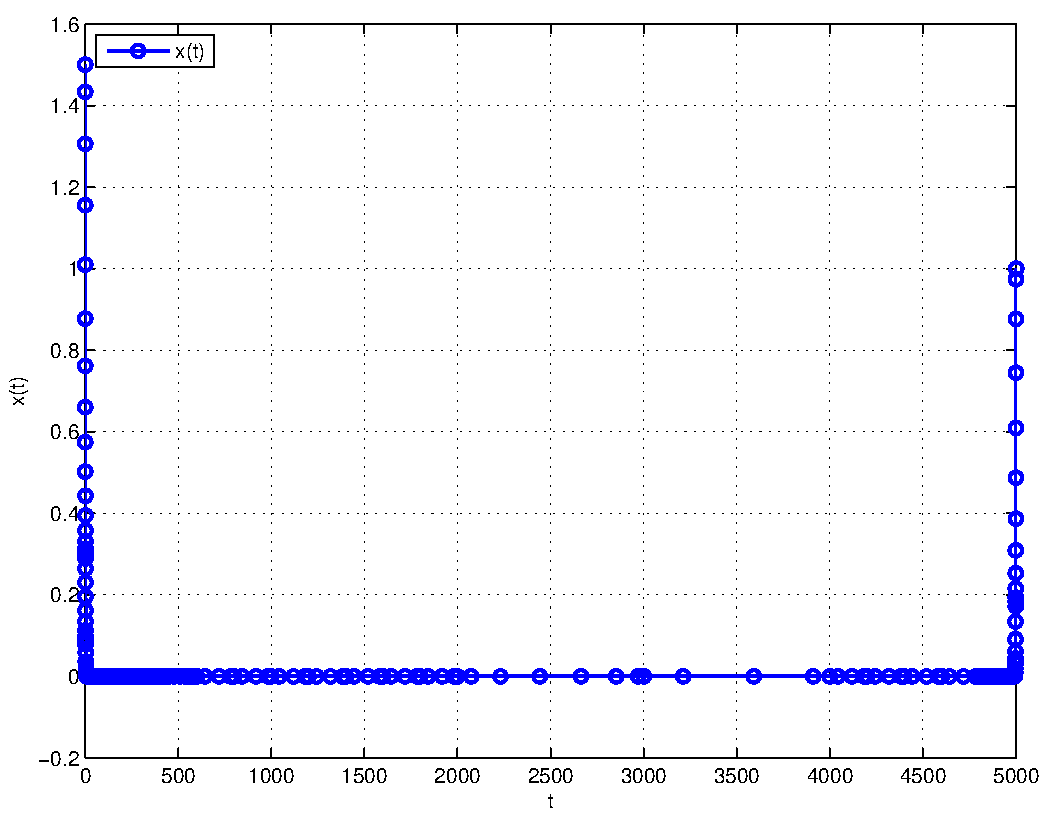
\includegraphics[scale=0.45]{HyperState.pdf}}~~~~~\subfloat[Control, $u(t)$, vs.~$t$. \label{fig:HyperControl}]{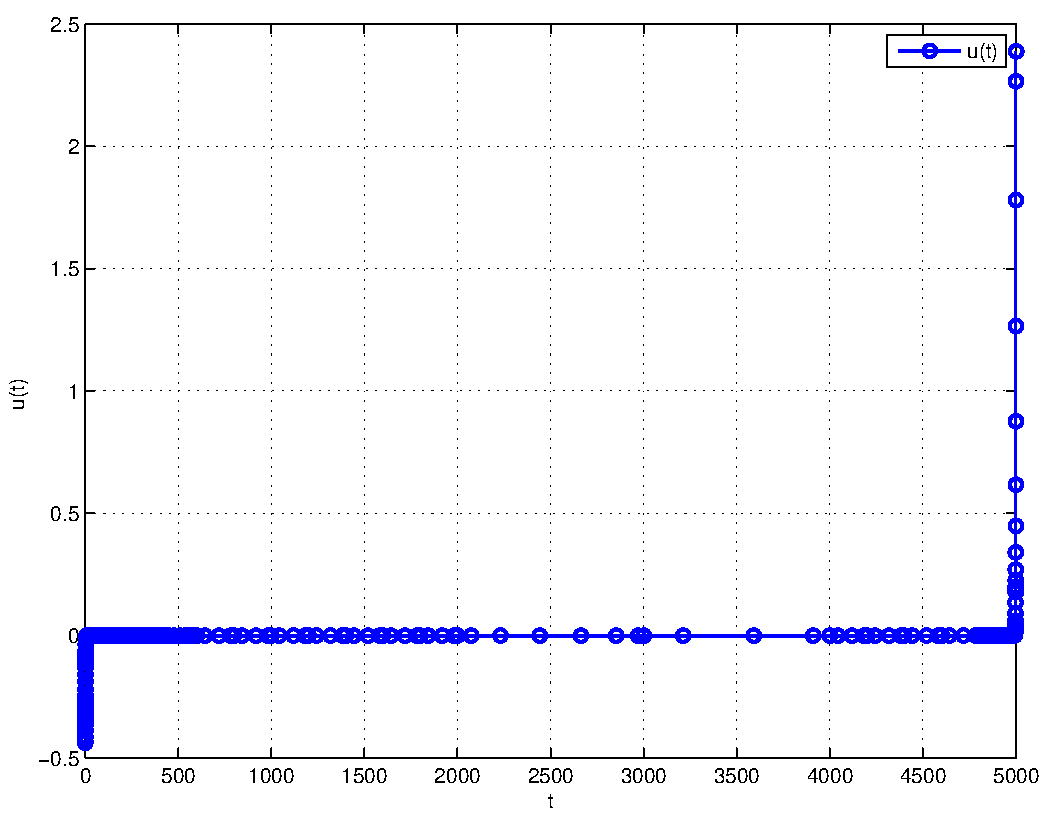
\includegraphics[scale=0.45]{HyperControl.pdf}}
		
		\subfloat[Costate, $\lambda(t)$, vs.~$t$. \label{fig:HyperCostate}]{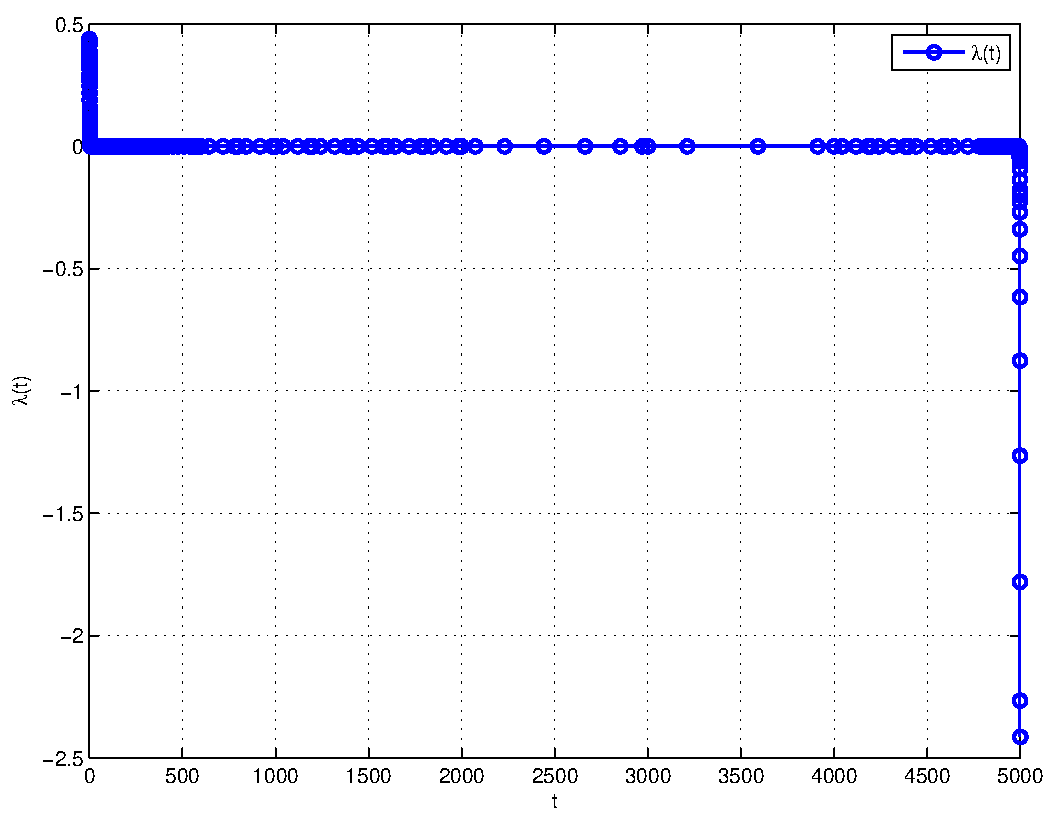
\includegraphics[scale=0.45]{HyperCostate.pdf}}
	\end{figure}
	\clearpage
	\subsection{Bryson-DenHam Problem}
	Consider the following optimal control problem.This problem is known in the literature as the Bryson-Denham problem\cite{bryson1969energy}.  Minimize the cost functional
	\begin{equation}
	J = x_3(t_f)
	\end{equation}
	subject to the dynamic constraints
	\begin{equation}
	\begin{array}{lcl}
	\dot{x_1} & = & x_2 \\
	\dot{x_2} & = & u \\
	\dot{x_3} & = & \frac{1}{2}u^2
	\end{array}
	\end{equation}
	the path constraint
	\begin{equation}
	0 \leq x_1(t) \leq 1/9
	\end{equation}
	and the boundary conditions
	\begin{equation}
	\begin{array}{lcl}
	x_1(0) & = & 0 \\
	x_2(0) & = & 1 \\
	x_3(0) & = & 0 \\
	x_1(t_f) & = & 0 \\
	x_2(t_f) & = & -1 \\
	\end{array}
	\end{equation}
	The \LPOPC code that solves this problem is shown below.\\
	\lstinputlisting{../example/bryson-denham/BrysonDenham.h}
	\lstinputlisting{../example/bryson-denham/BrysonDenham.cpp}
	\begin{figure}[h]
		\centering
		\subfloat[State vs.~Time.\label{fig:BrysonState}]{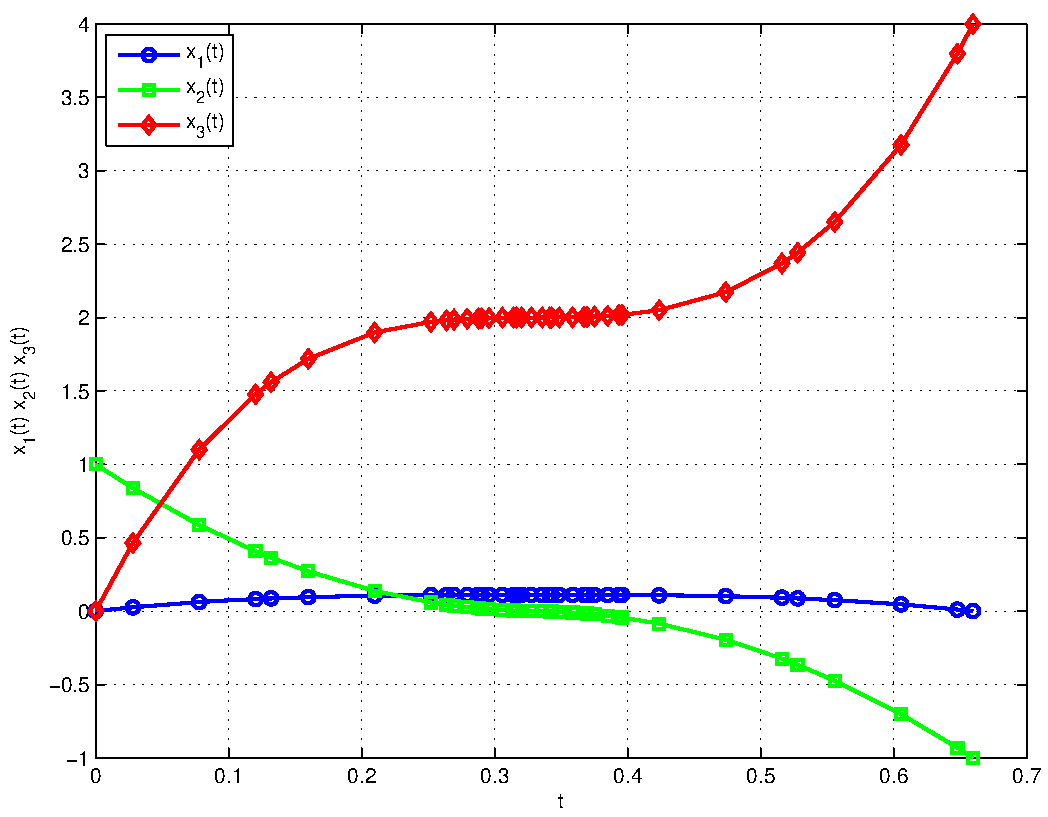
\includegraphics[scale=0.45]{BrysonState.pdf}}~~~~~\subfloat[Control vs.~Time. \label{fig:BrysonControl}]{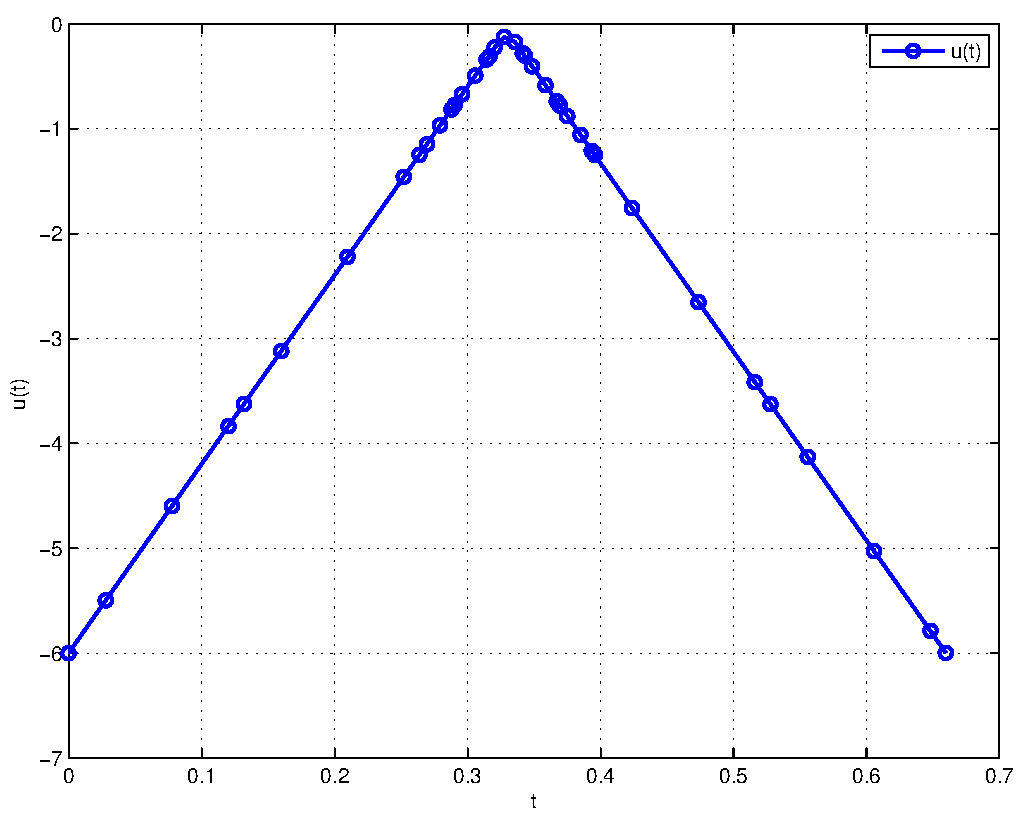
\includegraphics[scale=0.45]{BrysonControl.pdf}}
		
		\subfloat[Costate vs.~Time.\label{fig:BrysonCostate}]{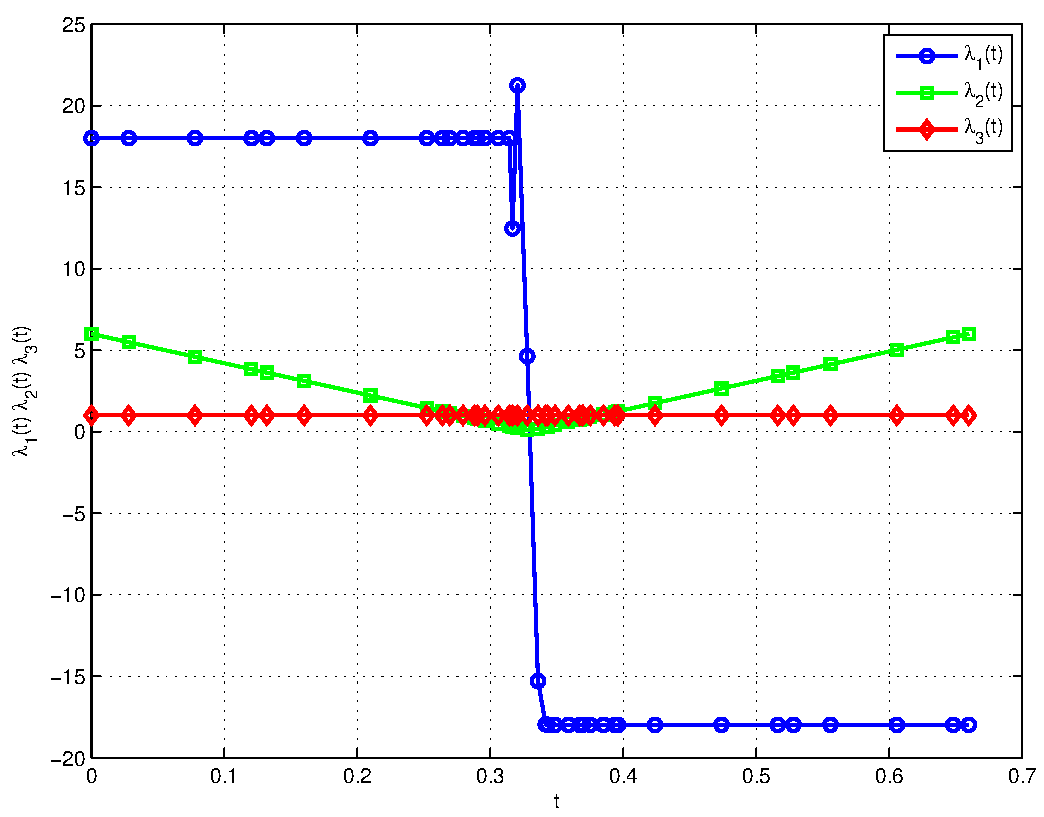
\includegraphics[scale=0.45]{BrysonCostate.pdf}}
	\end{figure}
	\clearpage
	\subsection{Launch}
	This problem consists of the launch of a space vechicl.See\cite{benson2005gauss}for a full description of the problem.\\Only a brief description is given here.The flight of the rocket can be divided  into four phases,with dry masses ejected from the vehicle at the end of phases 1,2 and 3.The final times of phase 1,2 and  3 are fixed,while the final time of phase 4 is free.
	The optimal control problem is then to find the control, ${ u}$,
    that minimizes the cost function
    
    \begin{equation}
    J=-m^{(4)}(t_f)
    \end{equation}
    
	The equations of motion for a non-lifting point mass in flight over a
	spherical rotating planet are expressed in Cartesian Earth centered inertial
	(ECI) coordinates as
	\begin{equation}\label{dyncs}
	\begin{array}{rcl}
	\dot{\textbf{r}} &=& { v} \vspace{3pt}\\
	\dot{\textbf{v}} &=& -\displaystyle\frac{\mu}{\|\textbf{r}\|^3}{ r} +
	\displaystyle\frac{T}{m}{ u} + \displaystyle\frac{{ D}}{m}  \vspace{3pt}\\
	\dot{m} & = & -\displaystyle\frac{T}{g_0I_{sp}}
	\vspace{3pt}\\
	\end{array}
	\end{equation}
	where ${ r}(t)=\left[\begin{array}{ccc} x(t) & y(t) & z(t)\end{array}\right]^T$
	is the position, ${ v} = \left[\begin{array}{ccc} v_x(t) & v_y(t) & v_z(t)\end{array}\right]^T$
	is the Cartesian ECI velocity, $\mu$ is the gravitational parameter, $T$ is
	the vacuum thrust, $m$ is the mass, $g_0$ is the acceleration due to gravity at sea level,
	$I_{sp}$ is the specific impulse of the engine,
	${ u} = \left[\begin{array}{ccc} u_x & u_y & u_z \end{array}\right]^T$ is the thrust
	direction, and ${ D}=\left[\begin{array}{ccc} D_x & D_y & D_z \end{array}\right]^T$
	is the drag force.  The drag force is defined as
	\begin{equation}
	{ D} = -\frac{1}{2}C_D A_{ref}\rho \|{ v}_{rel}\|{ v}_{rel}
	\end{equation}
	where $C_D$ is the drag coefficient, $A_{ref}$ is the reference area, $\rho$
	is the atmospheric density, and ${ v}_{rel}$ is the Earth relative
	velocity, where ${ v}_{rel}$ is given as
	\begin{equation}
	{ v}_{rel} = { v}-\boldsymbol{\omega} \times { r}
	\end{equation}
	where $\boldsymbol\omega$ is the angular velocity of the Earth relative to
	inertial space.  The atmospheric density is modeled as the exponential
	function
	\begin{equation}
	\rho = \rho_0\mbox{exp}[-h/h_0]
	\end{equation}
	where $\rho_0$ is the atmospheric density at sea level, $h=\| r\|-R_e$ is
	the altitude, $R_e$ is the equatorial radius of the Earth, and $h_0$ is the
	density scale height.  

	The launch vehicle starts on the ground at rest (relative to the Earth) at time $t_0$, so that the ECI initial conditions are
	\begin{equation}\label{ICs}
	\begin{array}{rcl}
	{ r}(t_0) &=& { r}_0 = \left[ \begin{array}{ccc} 5605.2 & 0 & 3043.4 \end{array} \right] ^T\quad \mbox{km} \vspace{3pt}\\
	{ v}(t_0) &=& { v}_0 = \left[ \begin{array}{ccc} 0 & 0.4076 & 0 \end{array} \right]^T \quad \mbox{km/s} \vspace{3pt}\\
	m(t_0) &=& m_0 = 301454 \quad \mbox{kg}
	\end{array}
	\end{equation}
	which corresponds to the Cape Canaveral launch site.  The terminal constraints
	define the target geosynchronous transfer orbit (GTO), which is defined in
	orbital elements as
	\begin{equation}\label{FCs}
	\begin{array}{rcl}
	a_f &=   &  24361.14 \; \mbox{km}, \\
	e_f &=   &  0.7308, \\
	i_f &=   &  28.5\deg,\\
	\Omega_f &= & 269.8\deg, \\
	\omega_f &= & 130.5\deg
	\end{array}
	\end{equation}
    A path constraint is imposed on the control to guarantee
	that the control vector is unit length, so that
	\begin{equation}\label{upath}
	|{ u}| = 1
	\end{equation}
	
  The following linkage constraints force the position and velocity to be continuous and also account for the mass ejections, as
	\begin{equation}
	\begin{array}{rcl}
	{ r}^{(p)}(t_f)-{ r}^{(p+1)}(t_0) &=& { 0}, \\
	{ v}^{(p)}(t_f)-{ v}^{(p+1)}(t_0) &=& { 0}, \qquad (p=1,\ldots,3)\\
	m^{(p)}(t_f)-m_{dry}^{(p)}-m^{(p+1)}(t_0) &=& 0 \\
	\end{array}
	\end{equation}
	where the superscript $(p)$ represents the phase number.\\
	
	The \LPOPC code that solves this problem is shown below.\\
	\lstinputlisting{../example/launch/Launch.hpp}
	\lstinputlisting{../example/launch/Launch.cpp}
	\begin{figure}[h]
		\centering
		\subfloat[Altitude vs.~Time.\label{fig:LaunchAltitude}]{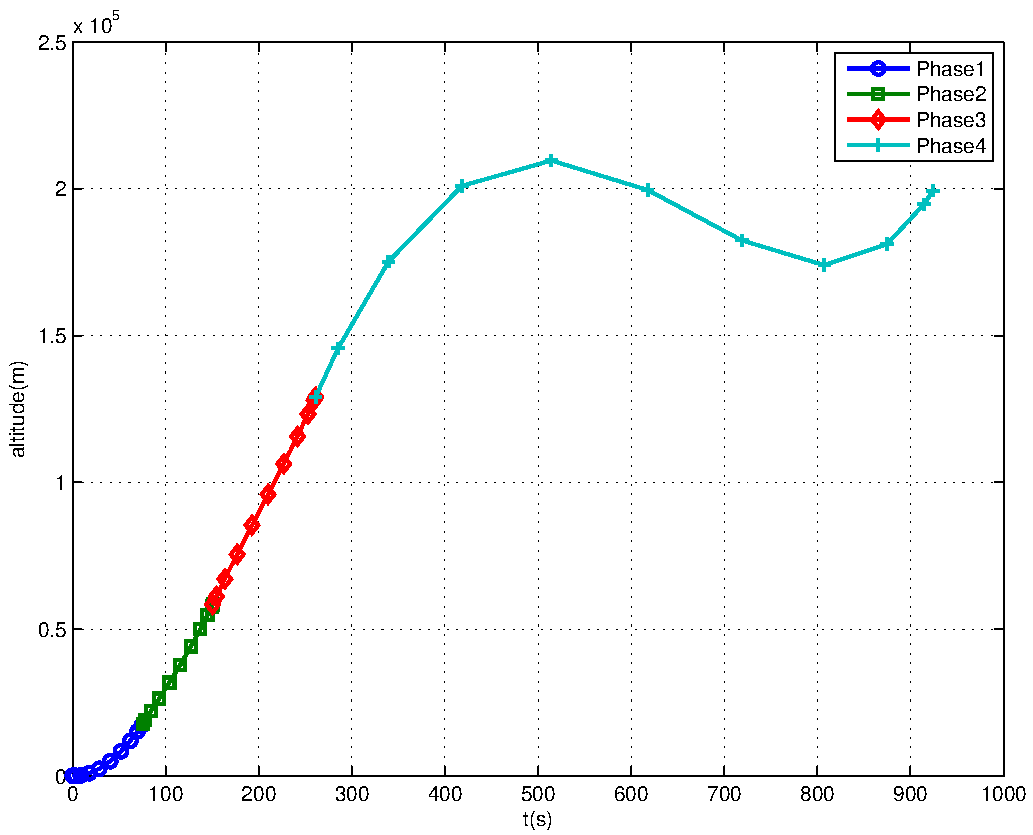
\includegraphics[scale=0.45]{LaunchAltitude.pdf}}~~~~~\subfloat[Speed vs.~Time. \label{fig:LaunchSpeed}]{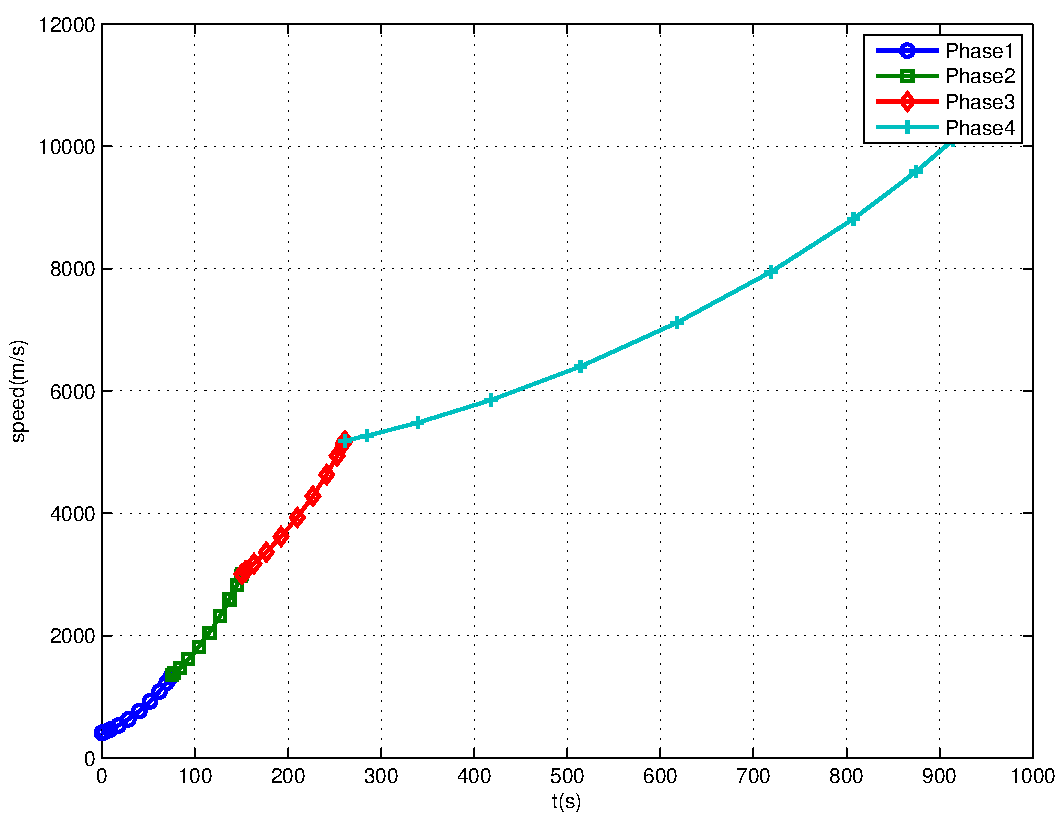
\includegraphics[scale=0.45]{LaunchSpeed.pdf}}
		
		\subfloat[Mass vs.~Time.\label{fig:LaunchMass}]{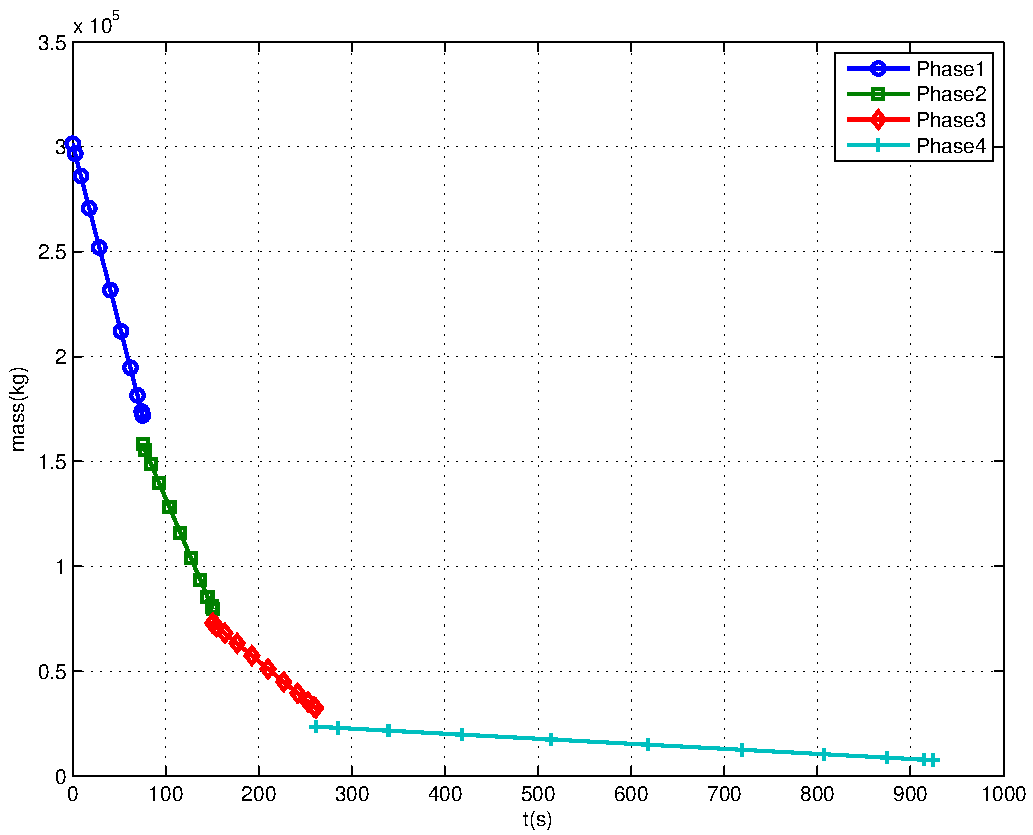
\includegraphics[scale=0.45]{LaunchMass.pdf}}~~~~~\subfloat[Control vs.~Time. \label{fig:LaunchControl}]{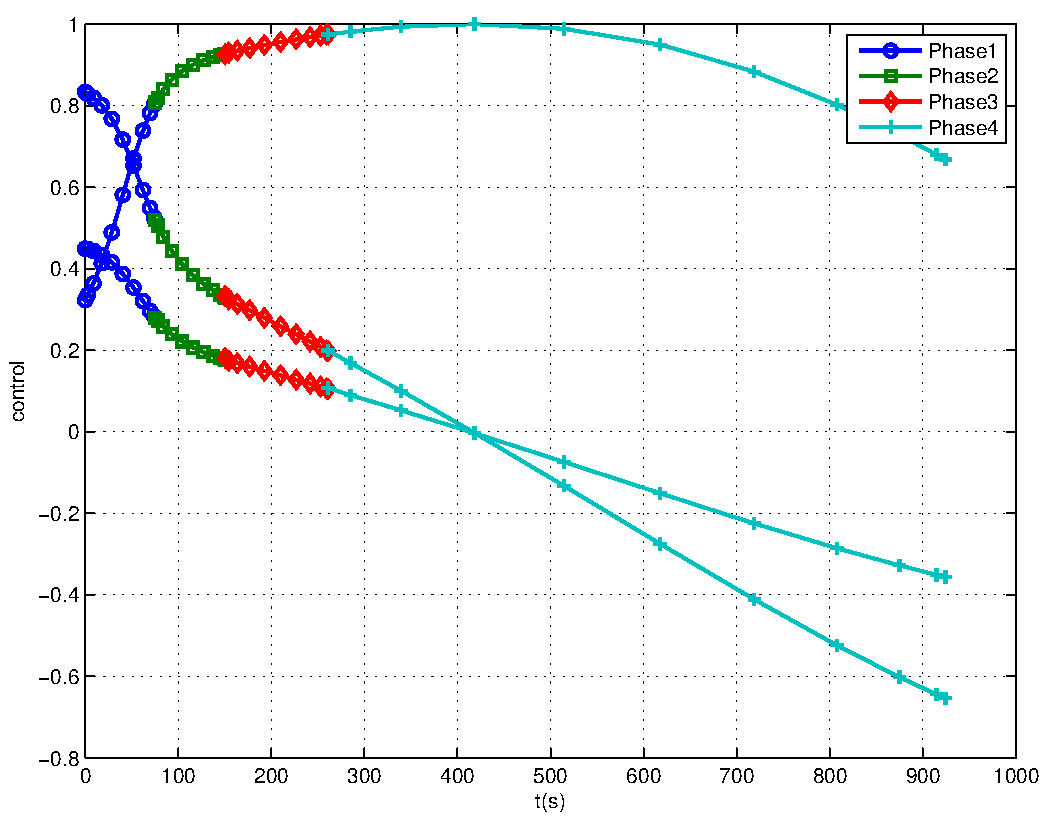
\includegraphics[scale=0.45]{LaunchControl.pdf}}
	\end{figure}
	\clearpage
\bibliography{lpref}
\end{document}
